%% =============================================================================
%% Natural Hazards (Springer) Manuscript — sn-jnl.cls (official template)
%% Springer Nature LaTeX template v3.x — Basic Springer Nature Reference Style
%% Target journal: Natural Hazards (Springer), ISSN 0921-030X / 1573-0840
%% Submit as ONE .tex file; figures attached separately.
%% =============================================================================
\documentclass[pdflatex,sn-basic]{sn-jnl}% Basic Springer Nature Reference Style

%% ── Standard packages (matching the official sn-article template) ──────────
\usepackage{graphicx}%
\usepackage{multirow}%
\usepackage{amsmath,amssymb,amsfonts}%
\usepackage[title]{appendix}%
\usepackage{xcolor}%
\usepackage{textcomp}%
\usepackage{manyfoot}%  required by sn-jnl.cls for footnote hooks
\usepackage{booktabs}%
\usepackage{array}%
\usepackage[caption=false,font=footnotesize]{subfig}%
\usepackage[section]{placeins}%  keep figures within their section
\usepackage[nolinks]{qrcode}%  QR code for the code/data repository
\usepackage{lineno}%  line numbers for peer review

%% ── Figures live in the shared project figures folder ─────────────────────
\graphicspath{{../figures/publication/}{./figures/}}
\DeclareGraphicsExtensions{.pdf,.png,.jpg}

%% ── Hyphenation ───────────────────────────────────────────────────────────
\hyphenation{gla-cial sus-cep-ti-bil-i-ty cor-dil-le-ra pro-gla-cial}

\raggedbottom

\begin{document}

%% =============================================================================
\title[A pan-Andean watch-list for glacial lake outburst floods]{%
  Pan-Andean explainable machine learning identifies priority glacial
  lakes for outburst flood early warning}

%% ── Authors ───────────────────────────────────────────────────────────────
\author*[1]{\fnm{Richar Andre} \sur{Vilca-Solorzano}}\email{75521963@est.unap.edu.pe}

\author[1]{\fnm{Dina Maribel} \sur{Yana-Yucra}}\email{maribelbel201314@gmail.com}

\author[1]{\fnm{Milton Vladimir} \sur{Mamani-Calisaya}}\email{mmamanic@unap.edu.pe}

\author[1]{\fnm{Fred} \sur{Torres-Cruz}}\email{ftorres@unap.edu.pe}

\affil*[1]{\orgdiv{Faculty of Statistical and Computer Engineering},
  \orgname{Universidad Nacional del Altiplano (UNAP)},
  \orgaddress{\city{Puno}, \country{Peru}}}

%% ── Abstract ──────────────────────────────────────────────────────────────
\abstract{Glacial lake outburst floods (GLOFs) threaten millions of people
across the Andes, yet disaster-risk managers lack scalable tools to
identify which lakes most urgently require field inspection. We present the
first pan-Andean GLOF susceptibility model that combines continental scale
with strict cross-national validation, interpretable physical drivers, and
an openly reproducible watch-list spanning Ecuador, Peru, Bolivia and
Chile. The model was trained on 20{,}140 unique glacial lakes derived from
69{,}643 multitemporal lake-year observations (Sentinel-2 and Landsat,
2017--2025) across fifteen regions in four countries. Of 71 compiled
historical GLOFs (1932--2023), 38 spatially matched the satellite
inventory, yielding 34 positive lake-years from 32 distinct source lakes
(1:629 class imbalance). Under strict lake-grouped out-of-fold
cross-validation, a Random Forest achieved the highest discrimination
(ROC-AUC\,=\,0.828; 95\%~CI: 0.729--0.916; permutation $p<0.001$).
Leave-One-Country-Out validation confirmed geographic transferability
(held-out Peru: ROC-AUC\,=\,0.80; Chile\,=\,0.72). SHAP analysis revealed
that GLOF-source lakes are distinguished by a multivariate signature of
moderate size, high compactness, low dam freeboard and proximity to
retreating ice. A compact top-2\% watch-list (403 lakes) recovers 41\% of
all confirmed GLOF-source lakes at 20.3$\times$ random precision (rising to
50\% in the top 5\%). After isotonic calibration the scores are reliable
(Brier skill score\,=\,0.24). By converting freely available satellite
data into an openly reproducible, ranked watch-list, this framework
provides resource-constrained Andean authorities with an actionable tool to
prioritize field inspection and protect downstream communities under
accelerating glacier retreat.}

\keywords{Glacial lake outburst flood, GLOF susceptibility, Explainable
machine learning, SHAP interpretability, Disaster risk reduction, Andes}

\maketitle

\linenumbers

%% =============================================================================
\section{Introduction}\label{sec:intro}

The tropical and subtropical Andes host approximately 99\% of the
world's tropical glaciers \citep{Rabatel2013}, which are retreating at
accelerating rates under anthropogenic climate change
\citep{Zemp2019,Hugonnet2021,GlaMBIE2025}. Andean glaciers have lost
roughly 30\% of their volume since the 1980s, with mass-loss rates
accelerating through the 2010s \citep{Dussaillant2019,Masiokas2020}. A
direct consequence is the rapid proliferation and enlargement of
proglacial and moraine-dammed lakes \citep{Haeberli2017,Shugar2020,
Wood2021,Carrivick2013}, which constitute the primary source of GLOF hazard across
the entire mountain range \citep{Rounce2024,Emmer2017,EmmerHarrison2020,Zheng2021}.

GLOFs pose acute risks to downstream communities across four countries.
In \textit{Peru}, the deadliest recorded GLOF occurred in 1941 when
Laguna Palcacocha (Cordillera Blanca) released approximately
$10{\times}10^6$~m$^3$ of water, killing an estimated 5{,}000 people in
Huaraz \citep{Carey2010}. Socio-economic losses from glacier retreat and
associated hazards in the Cordillera Blanca amount to hundreds of
millions of dollars over recent decades
\citep{Motschmann2020,Bury2011,Baraer2012}. In \textit{Bolivia}, the
rapid disappearance of tropical glaciers such as Chacaltaya threatens
freshwater supply to La Paz and El Alto, while moraine-dammed lakes in
the Cordillera Real generate persistent GLOF hazard
\citep{Francou2003,Rabatel2006}. In \textit{Ecuador}, glaciers on
Antisana, Cotopaxi, and Chimborazo have retreated dramatically since
the 1950s \citep{Caceres2010,Veettil2019}, and glacial lake outbursts
pose risk to densely populated Andean valleys. In \textit{Chile},
moraine-dammed lake failures in Patagonia and the Andes Centrales have
caused repeated infrastructure damage
\citep{IribarrenAnacona2014,IribarrenAnacona2015}. Globally, an
estimated 15 million people are directly exposed to GLOF impacts
\citep{Taylor2023}, and GLOF frequency has increased across most
glacierized mountain regions during the twentieth century
\citep{Lutzow2023,Veh2022,Veh2023,Zheng2021}. The economic costs of rapid glacier retreat
across the Andes are substantial and growing
\citep{Vergara2007,Immerzeel2010,Immerzeel2020}, creating urgent demand
for scalable, data-driven susceptibility tools to support disaster risk
reduction (DRR).

Despite the growing hazard, existing GLOF susceptibility studies in
the Andes have predominantly focused on single cordilleras
\citep{Emmer2020,EmmerHarrison2020,McKillop2007} or relied on
morphometric scoring schemes lacking rigorous statistical validation
\citep{Emmer2016,Hegglin2008,Frey2010}. Glacial lake mapping from
satellite imagery has advanced substantially with Sentinel-2 time
series \citep{Sentinel2MSI,Wangchuk2020}, yet continent-scale
susceptibility models with explicit geographic cross-validation
remain rare \citep{IribarrenAnacona2014}. A community-wide review
identified validated susceptibility modelling and geographic
transferability as the most critical open challenges in GLOF research
\citep{Pronk2022}. To our knowledge, no prior GLOF susceptibility model
has combined continental spatial scale with strict cross-national
geographic validation: existing quantitative models are confined to a
single cordillera or country and are validated on random train--test
splits, leaving open the central question of whether a model learned in one
range transfers to another. Machine learning has emerged as the leading
approach for natural hazard susceptibility mapping
\citep{Merghadi2020,Pourghasemi2020,Ghorbanzadeh2019}, but its
application to GLOFs under extreme class imbalance and data-scarce
conditions has seldom been rigorously evaluated \citep{He2009}.

This study addresses these gaps with four principal contributions:
(1)~the first harmonized, multitemporal glacial lake inventory (2017--2025)
covering fifteen regions across four Andean countries---from the tropical
cordilleras to Patagonia---at continental scale from Sentinel-2 and Landsat
imagery; (2)~a machine learning susceptibility
model evaluated under strict out-of-fold (OOF) cross-validation with rigorous
Leave-One-Country-Out (LOCO) geographic validation, establishing transferability
across distinct Andean glaciological and climatic settings;
(3)~SHAP-based physical interpretation linking susceptibility to
observable glaciological and geomorphological controls, evaluated through
complementary non-parametric significance procedures; and
(4)~a fully open-source, reproducible pipeline enabling direct application
and extension to other glacierized mountain regions, in support of
operational disaster risk reduction.

%% =============================================================================
\section{Related work}\label{sec:related}

\subsection{GLOF susceptibility modelling}

Quantitative GLOF susceptibility assessment has evolved from
expert-based morphometric scoring \citep{McKillop2007,Emmer2016,Richardson2000} to
statistical and machine learning approaches. \citet{McKillop2007} applied logistic regression to 174 moraine-dammed
lakes in British Columbia, achieving ROC-AUC\,=\,0.77 but relying on a
random train--test split without geographic stratification. Rounce et
al.\ \citep{Rounce2017} proposed a random-forest framework for Nepal
achieving AUC\,=\,0.81, yet limited to a single mountain system.
\citet{Cook2016} assessed GLOF susceptibility in the
Bolivian Andes combining glacier change data with multi-criteria
analysis, without statistical learning or cross-national validation.
\citet{Allen2016} developed an integrative GIS-based
GLOF hazard framework for India incorporating both current and future
threats under glacier retreat scenarios. Emmer
et al.\ \citep{Emmer2020} assessed 232 glacial lakes in the Cordillera
Blanca using logistic regression (AUC\,=\,0.80), the most comprehensive
Andean study to date but restricted to a single cordillera. Wilson et
al.\ \citep{Wilson2018} provided a detailed geomorphological analysis of
a moraine-dammed lake failure in the Patagonian Andes, while Iribarren
Anacona et al.\ \citep{IribarrenAnacona2014} assessed outburst
susceptibility for moraine-dammed lakes in the Chilean Baker basin
using a multi-criteria scoring approach; \citet{Kougkoulos2018} applied multi-criteria decision analysis to
identify potentially dangerous glacial lakes globally. \citet{Sattar2022} analysed moraine-to-ice-dam lake transitions in the
Karakoram, underscoring dam-type complexity without providing a
continental-scale susceptibility model. Across this body of work, none
of the cited studies employed Leave-One-Country-Out (LOCO) validation
or covered more than one national territory, leaving cross-national
model transferability unanswered \citep{Pronk2022}.

\subsection{Machine learning for glacial and cryospheric hazards}

Machine learning has been extensively applied to landslide and flood
susceptibility mapping \citep{Merghadi2020,Pourghasemi2020} and to
extreme climate hazard prediction in high-altitude Andean environments
\citep{Torres-Cruz2025}, but its adoption in glacial hazard assessment
remains limited. The central
challenge in GLOF modelling is extreme class imbalance: documented GLOF
events typically represent less than 0.5\% of all glacial lakes in any
inventory \citep{Rounce2024,Lutzow2023}, making conventional accuracy
metrics misleading \citep{Lobo2008,Chicco2020,He2009}. Balanced
resampling methods---particularly Balanced Random Forest \citep{Chen2004}
and EasyEnsemble \citep{Liu2009}---have demonstrated superior
performance to SMOTE-based oversampling under severe imbalance ratios
\citep{Lemaitre2017}, yet their application in pan-regional GLOF
assessment has not previously been validated. Explainable AI approaches
(SHAP) \citep{LundbergLee2017,Lundberg2020} provide model-agnostic
interpretability critical for translating ML predictions into
physically meaningful susceptibility drivers, bridging the gap between
black-box performance and operational glaciological knowledge
\citep{Merghadi2020,Ghorbanzadeh2019}.

\subsection{Remote sensing of glacial lakes}

Sentinel-2 (launched 2015) provides 10~m multispectral imagery at
five-day revisit frequency \citep{Sentinel2MSI}, enabling systematic
monitoring of glacial lakes at unprecedented spatial and temporal
resolution. The Modified Normalized Difference Water Index
(MNDWI\,=\,$(B_3-B_{11})/(B_3+B_{11})$) \citep{Xu2006}, building on
the original NDWI \citep{McFeeters1996}, has become the standard for
open water delineation in optically complex glacial environments.
\citet{Wangchuk2020} demonstrated that Sentinel-1
and Sentinel-2 fusion outperforms single-sensor approaches for glacial
lake mapping in cloud-prone regions; the same group later extended this
to GLOF susceptibility monitoring with persistent scatterer
interferometry \citep{Wangchuk2022}, a finding particularly relevant
for the tropical Andes. Global surface water monitoring using Landsat imagery
\citep{Pekel2016,Shugar2020,Wang2020} documented a 51\% increase in global
glacial lake area between 1990 and 2018, with accelerating growth in
Andean systems \citep{Drenkhan2019,Colonia2017}. However,
continent-scale Sentinel-2 multitemporal inventories covering the full
Andean arc remain unpublished, motivating the present work.

%% =============================================================================
\section{Methodology}\label{sec:methods}

\subsection{Study area}

The study encompasses fifteen glacial regions spanning a latitudinal
range of $0.3^\circ$N to roughly $47^\circ$S across four countries
(Fig.~\ref{fig:study_area}; Table~\ref{tab:study_areas}). The
selection covers the full spectrum of tropical, subtropical and
extratropical Andean glaciological settings, from the heavily glacierized
Cordillera
Blanca---home to 27\% of the world's tropical glaciers
\citep{Rabatel2013}---to the Mediterranean-climate Andes Centrales in
central Chile \citep{Masiokas2020}.

\textbf{Peru (seven cordilleras):} Cordillera Blanca ($8$--$10^\circ$S)
is the most extensively studied system, containing the largest
concentration of tropical glaciers worldwide and historically the most
GLOF-affected range in the Andes
\citep{Emmer2022,EmmerHarrison2020,Carey2012}. Cordilleras Huayhuash (including the 2023 Lago~Rasac GLOF
\citep{Emmer2025}), Raura, Vilcanota, Central, Urubamba, and Huanzo
complete the Peruvian coverage, representing diverse glaciological and
socio-hydrological contexts \citep{Bury2011,Baraer2012,Drenkhan2019,Colonia2017}.

\textbf{Bolivia (Cordillera Real):} The Cordillera Real
($15$--$17^\circ$S) encompasses the main glacierized range of Bolivia,
with glaciers feeding freshwater to La Paz and El Alto
\citep{Immerzeel2020}. This system has experienced dramatic glacier
retreat since the 1980s \citep{Francou2003,Soruco2009}, generating new
proglacial lakes with growing GLOF potential.

\textbf{Ecuador (Antisana complex):} The Antisana volcanic complex
($0.3^\circ$N--S) hosts glaciers on steep volcanic flanks at high
elevation \citep{Caceres2010,Vuille2018}. Glacial lake formation is
controlled by the interaction between volcanic topography and rapid ice
retreat \citep{Veettil2019}.

\textbf{Chile (Andes Centrales):} The Andes Centrales
($33$--$35^\circ$S) represent the southernmost and climatically
distinct study region, where Mediterranean seasonality drives a
different lake-formation regime \citep{Masiokas2020,IribarrenAnacona2014}.
No historical GLOF events were matched in this region, providing an
important null-class validation domain.

Figure~\ref{fig:iconic} shows Sentinel-2 true-colour imagery of three
confirmed GLOF-source lakes spanning the Peruvian cordilleras---Laguna
Palcacocha (the 1941 Huaraz disaster), Lake~513 (2010), and Laguna
Rasac (2023)---all of which the model independently classifies as
high-susceptibility.

\begin{figure}[htbp]
\centering
\includegraphics[width=\textwidth,keepaspectratio]%
  {fig9_iconic_lakes.jpg}
\caption{Sentinel-2 true-colour imagery (bands B4--B3--B2, dry-season
  composites) of three confirmed GLOF-source lakes in the Peruvian
  Andes. Each panel reports the recorded outburst event and the
  model-predicted susceptibility class (HIGH if above the Youden
  threshold $t\!\approx\!0.39$). Imagery: ESA Copernicus via Google Earth
  Engine.}
\label{fig:iconic}
\end{figure}

\begin{figure}[htbp]
\centering
\includegraphics[width=\textwidth,height=0.55\textheight,keepaspectratio]%
  {fig1_susceptibility_map.jpg}
\caption{Pan-Andean glacial lake GLOF susceptibility overview map.
  Glacial lakes are plotted across fifteen study regions from the tropical
  Andes to Patagonia; colour encodes predicted susceptibility score
  (blue\,=\,low; red\,=\,high); point size scales with
  $\log(\mathrm{area})$. Stars ($\star$) mark the 71 historical GLOF events
  (1932--2023); open circles denote study-area centroids. Inset: location
  of the study region within South America (red rectangle). Detailed zoom
  maps for the study areas are presented in Appendix~\ref{app:area_maps}.
  Shaded-relief basemap: Esri World Shaded Relief; country outlines:
  Natural Earth.}
\label{fig:study_area}
\end{figure}

\begin{table}[!t]
\caption{Summary of the fifteen study regions, grouped by country.
  $n_\text{lakes}$: unique modelled lakes ($\geq$\,0.05~km$^2$,
  multitemporal record collapsed to physical lakes).
  $n_\text{GLOF}$: matched historical source lake-years. High-risk\,\%:
  proportion above the Youden threshold ($t\!\approx\!0.39$) from lake-grouped
  out-of-fold Balanced Random Forest predictions. The 71 compiled events
  matched 34 source lake-years (32 distinct lakes).}
\label{tab:study_areas}
\centering
\begin{tabular*}{\textwidth}{@{\extracolsep{\fill}}llccc}
\toprule
\textbf{Region} & \textbf{Country} & \textbf{$n_\text{lakes}$}
  & \textbf{$n_\text{GLOF}$} & \textbf{High-risk (\%)} \\
\midrule
Raura            & Peru    &   550 & 6 & 46.0 \\
Huayhuash        & Peru    &   309 & 2 & 46.6 \\
Central          & Peru    &   200 & 0 & 71.0 \\
Carabaya         & Peru    &   275 & 1 & 37.5 \\
Urubamba         & Peru    &   343 & 4 & 32.7 \\
Apolobamba       & Bolivia &   556 & 0 & 21.0 \\
Vilcanota        & Peru    & 1{,}383 & 3 & 36.8 \\
Blanca           & Peru    & 1{,}237 & 3 & 35.2 \\
Antisana         & Ecuador &   229 & 4 & 48.5 \\
Real             & Bolivia &   122 & 1 & 27.0 \\
Huanzo           & Peru    &    52 & 1 & 50.0 \\
Andes Centrales  & Chile   & 5{,}030 & 3 & 16.3 \\
Patagonia Norte  & Chile   & 7{,}236 & 5 &  6.5 \\
Patagonia Sur    & Chile   & 2{,}614 & 1 &  5.4 \\
Bolivia Norte    & Bolivia &     4 & 0 & 50.0 \\
\midrule
\textbf{Total} &  & \textbf{20{,}140} & \textbf{34} & \textbf{17.0} \\
\bottomrule
\end{tabular*}
\end{table}

\subsection{Input datasets and data sources}

Table~\ref{tab:data_sources} summarizes the four primary datasets.
Sentinel-2 Level-2A (surface reflectance) imagery was accessed and
composited via Google Earth Engine \citep{Gorelick2017}. Digital elevation data were sourced
from NASADEM Merged DEM (NASA EARTHDATA, 30~m; \citep{NASADEM2020}).
Glacier outlines were obtained from the Randolph Glacier Inventory
v7.0 (RGI~7.0; \citep{RGI2023}), and the historical GLOF inventory
was compiled from four open sources: GloFLOD \citep{Lutzow2023}, the
tropical Andes inventory \citep{Emmer2022}, INAIGEM official records
\citep{INAIGEM2018}, and \citet{IribarrenAnacona2015}.

\begin{table}[!t]
\caption{Primary input datasets, providers, and access conditions.}
\label{tab:data_sources}
\centering
\begin{tabular*}{\textwidth}{@{\extracolsep{\fill}}llcc}
\toprule
\textbf{Dataset} & \textbf{Source} & \textbf{Res.} & \textbf{Access} \\
\midrule
Sentinel-2 L2A (2017--2025) & ESA Copernicus  & 10~m   & Free \\
Landsat C2 L2 (2017--2025)   & USGS/NASA       & 30~m   & Free \\
NASADEM Merged DEM           & NASA EARTHDATA  & 30~m   & Free \\
RGI v7.0 glacier outlines    & GLIMS/NSIDC     & Vector & Open \\
GLOF inventory (71 events; 38 matched) & GloFLOD+INAIGEM & Point & Open \\
\bottomrule
\end{tabular*}
\end{table}

\subsection{Glacial lake inventory}

Glacial lake boundaries were delineated from annual Sentinel-2 L2A
composites for 2017--2025. Cloud-free scenes were selected for the
austral dry season (June--September in the Southern Hemisphere;
December--March in Ecuador). Surface water was extracted using the
Modified Normalized Difference Water Index
(MNDWI\,=\,$(B_3-B_{11})/(B_3+B_{11})$; \citep{Xu2006,McFeeters1996}),
with a threshold of 0.0, complemented by morphological filtering to
remove river channels and ephemeral water bodies. Lakes were retained
if their area exceeded 1{,}000~m$^2$ and if located within 5~km of
glacier outlines from RGI~7.0 \citep{RGI2023}. Annual delineations
were aggregated into a unified database, yielding 69{,}643 lake-year
observations (Fig.~\ref{fig:database}); for modelling, the multitemporal
record was collapsed to unique physical lakes and restricted to
substantial water bodies ($\geq$\,0.05~km$^2$), giving 20{,}140 lakes.
Table~\ref{tab:qc_inventory} summarises the six quality-control criteria
applied consistently across all fifteen study regions.

\begin{table}[!t]
\caption{Lake inventory quality-control protocol applied uniformly across
  all fifteen regions. Each criterion was applied in the order listed.}
\label{tab:qc_inventory}
\centering
\begin{tabular*}{\textwidth}{@{\extracolsep{\fill}}llp{4.2cm}}
\toprule
\textbf{Step} & \textbf{Criterion} & \textbf{Value / Rule} \\
\midrule
1. Spectral index & MNDWI threshold & $\geq 0.0$ (Xu, 2006) \\
2. Minimum size   & Area filter      & $\geq 1{,}000$~m$^2$ \\
3. Channel removal & Morphological opening & Eliminate linear water bodies \\
4. Glacial origin  & RGI~7.0 proximity & $\leq 5{,}000$~m from glacier outline \\
5. Seasonality     & Scene composite   & Jun--Sep (SH); Dec--Mar (Ecuador) \\
6. Multi-year      & Annual delineation & 2017--2025; $\geq 1$ valid scene/year \\
\bottomrule
\end{tabular*}
\end{table}

\subsection{Inventory validation}

The automated inventory comprises 69{,}643 lake-year observations from
roughly 55{,}700 distinct lakes. Its size-frequency distribution is
dominated by small water bodies (median area $\approx$\,2~ha; 65\% below
5~ha; 35\% below 1~ha), in agreement with the strongly right-skewed size
distributions
reported for Andean and global glacial-lake inventories
\citep{Shugar2020,Wood2021,Drenkhan2019}, and the documented total
lake-area growth over 2017--2025 (Fig.~\ref{fig:database}a) is
consistent with regional glacier-retreat trends
\citep{Dussaillant2019,GlaMBIE2025}. A minor tail of larger polygons
reflects residual commission of non-glacial water bodies (e.g.\
reservoirs and bedrock lakes) that fall within the glacier buffer.
Importantly, such commission is \emph{not} self-correcting: because lake
size is itself strongly associated with the predicted score (Spearman
$\rho\!=\!0.65$ between log-area and score), large commission
polygons tend to receive elevated rather than negligible scores---of
507 large ($>$5~ha), glacier-distal ($>$5~km) lake-years, the median
predicted score is 0.69. Glacier proximity, the leading SHAP predictor,
only partially offsets this ($\rho\!=\!-0.34$ with score). Residual
commission therefore has the potential to inflate the
high-susceptibility count and even the operational watch-list, so
screening out non-glacial water bodies---via the very-high-resolution
protocol specified below---is a necessary pre-deployment step rather
than an optional refinement.

Automated MNDWI delineation can also produce gross errors---multi-part
geometries where the water mask merges a lake with adjacent rivers, wet
ground, or terrain shadow---and we therefore cap lake area within the
detection pipeline and discard implausibly large or fragmented polygons.
Critically, the prioritization is not sensitive to residual size errors:
the interpretability analysis (\S\,\ref{sec:stats}) shows that GLOF-source
lakes are \emph{not} the largest water bodies but are distinguished by a
multivariate signature of shape, dam freeboard and glacier context, so
that over-delineated polygons may inflate the absolute high-risk count but
do not drive the ranking. Stricter geometric quality control (compactness
and maximum-area filters, or single-component re-delineation) is
nonetheless recommended before operational deployment. A formal omission/commission accuracy
assessment was not performed against an independent reference, which is a
limitation (\S\,\ref{sec:limitations}); we therefore specify a
reproducible validation protocol for future work and revision: a
stratified random sample of $\geq\!50$ lakes per cordillera, manually
photo-interpreted against very-high-resolution imagery (PlanetScope or
Google Earth) by an independent operator, scored for omission and
commission to report producer's/user's accuracy and F1 per size class.

As a first quantitative bound pending this manual audit, we applied an
automated physiographic plausibility screen: a lake was flagged as
potentially non-glacial when it fell outside the physiographic envelope
occupied by the confirmed GLOF-source lakes---farther than their
95th-percentile ice distance (9.8~km) or below their 5th-percentile
elevation (2{,}900~m~a.s.l.). About 35\% of the modelled inventory
(7{,}063 of 20{,}140 lakes) fell outside this envelope and are candidate
commission or non-glacial features. Crucially, this fraction collapses
toward the operational thresholds: only 5.0\% of the top-2\% watch-list,
and 2.0\% of the top-0.5\%, are off-context, against 35.1\% at baseline---a
7--17-fold reduction. The prioritization therefore concentrates strongly on
physiographically plausible glacial lakes rather than being driven by
commission artefacts: the in-context (plausible) lakes carry a higher median
out-of-fold susceptibility (0.276) than the off-context lakes (0.188), so the
watch-list filters \emph{out} rather than \emph{in} the candidate
non-glacial features. This bounds---though does not replace---the
independent accuracy assessment specified above.

In the absence of an independent reference inventory, we quantify
detection reliability through \emph{multitemporal persistence}: because
cloud, shadow, and seasonal-snow artefacts do not recur at a fixed
location across independent annual composites, a lake re-detected in
several years is very unlikely to be spurious. Multi-year persistence is
highest precisely in the most GLOF-active tropical cordilleras---Cordillera
Central (39\% of lakes re-detected in $\geq\!2$ years), Raura (35\%),
Blanca (28\%) and Huayhuash (26\%)---so the lakes that matter most for
hazard triage are also the most reliably mapped, whereas the extratropical
regions, composited from fewer cloud-free scenes, show lower repeat
detection. Because susceptibility is scored on the multitemporal mean of
each physical lake rather than on any single year, the inventory is used as
a body of repeated observations rather than requiring per-lake persistence.
The conservative 1{,}000~m$^2$ minimum-area threshold and cloud-free
compositing keep the inventory consistent in order of magnitude with
national glacial-lake inventories \citep{Emmer2022,INAIGEM2018}.

\subsection{Feature engineering}

For each lake, 40 features were organized into six
groups (Table~\ref{tab:feature_groups}). Because tree ensembles are
insensitive to multicollinearity among predictors---unlike linear
models---correlated descriptors (for example, the four empirical depth
estimates, which are monotone transforms of area) were retained rather
than pruned; a Spearman correlation screen confirmed that no pair of
retained features was collinear to the point of numerical instability, and
the random splitting of features at each tree node further decorrelates
their use. The groups are:

\begin{enumerate}
\item \textbf{Morphometric (8):} area, perimeter, compactness,
  elongation, fractal dimension, convexity, equivalent diameter,
  and shoreline development index.
\item \textbf{Topographic (12):} mean, min, max, and std of elevation;
  mean and std of slope; aspect; terrain ruggedness index (TRI)
  \citep{Riley1999}; topographic wetness index; curvature; surface
  roughness; and a vector ruggedness measure.
\item \textbf{Dam and glacier context (4):} distance to the nearest
  glacier, dam elevation, dam freeboard, and dam height.
\item \textbf{Hydrological/depth (11):} depth estimates from four
  empirical area--depth scaling laws
  \citep{Huggel2002,Yao2012,CookQuincey2015,OConnor2001}, their
  ensemble mean and standard deviation, an Andes-corrected depth and its
  uncertainty, impounded volume, area-to-depth ratio, and potential
  energy.
\item \textbf{Temporal (4):} multi-year area trend, area coefficient of
  variation, detection presence rate, and annual growth rate
  (m$^2$\,yr$^{-1}$).
\item \textbf{Composite (1):} an aggregate risk index combining size,
  slope, and growth.
\end{enumerate}

Topographic descriptors (elevation, slope, slope variability, and
terrain ruggedness) were derived per lake as zonal statistics over each
lake footprint from 30~m NASADEM-derived rasters \citep{NASADEM2020},
and glacier distance from per-area distance-to-ice rasters built from
RGI~7.0 outlines.
Missing values were imputed with column-wise medians computed
exclusively from the training fold (no leakage from test data);
a secondary fill of zero was applied where the median was also
missing. Terrain features could be missing for the few lakes lying outside
DEM coverage; these cases were median-imputed within the training fold
rather than treated as structural data absence.

With 40 features and $n^+\!=\!32$ positive lakes, standard parametric
models risk overfitting. The tree ensembles mitigate this through per-tree
bootstrap resampling and random feature subsampling at each split, and the
leave-one-GLOF-out jackknife (\S\,\ref{sec:stats}) confirms that the
discriminative signal is not concentrated in any subset of positive labels.

\begin{table}[!t]
\caption{Feature groups and count for each lake.}
\label{tab:feature_groups}
\centering
\begin{tabular}{llc}
\toprule
\textbf{Group} & \textbf{Feature types} & \textbf{Count} \\
\midrule
Morphometric        & Shape, size, boundary indices       & 8 \\
Topographic         & DEM derivatives (elevation, slope)  & 12 \\
Dam \& glacier      & Glacier distance, dam geometry      & 4 \\
Hydro./depth        & Empirical depth laws, volume, energy & 11 \\
Temporal            & Annual areas, growth rates          & 4 \\
Composite           & Aggregate risk index                & 1 \\
\midrule
\textbf{Total} & & \textbf{40} \\
\bottomrule
\end{tabular}
\end{table}

\subsection{GLOF inventory and label assignment}

A historical GLOF inventory of 71 events (1932--2023) was compiled by
synthesizing GloFLOD \citep{Lutzow2023}, the tropical Andes inventory
\citep{Emmer2022}, INAIGEM records \citep{INAIGEM2018}, and Patagonian
events \citep{IribarrenAnacona2015}, following the GAPHAZ framework
\citep{GAPHAZ2017}. Positive labels ($y\!=\!1$) were assigned to
lake-year observations within a 5{,}000~m buffer of an inventory event;
38 of the 71 events matched the satellite inventory, yielding 34 positive
lake-year labels that collapse to 32 distinct source lakes among the
20{,}140 modelled (prevalence\,=\,0.0016; class ratio~1:629). The positive
set is essentially insensitive to the matching radius: widening the buffer
to 15~km recovers only three additional candidate events, all of which are
coordinate-error cases (reported impact points lying several kilometres
from any detected lake) rather than genuine new source lakes
(\S\,\ref{sec:limitations}). Although the positive class is small, the
bootstrap confidence interval already accounts for this sampling
variability (\S\,\ref{sec:stats}).
A leave-one-GLOF-out (jackknife) sensitivity analysis confirmed that
no single positive event drives discriminative performance: each held-out
GLOF lake received a mean susceptibility of 0.37 (range 0.00--0.94), far
above the 0.0016 base rate, so the discriminative signal is distributed
across the positive set rather than concentrated in any single event.

\subsection{Machine learning pipeline}\label{sec:pipeline}

Six classifiers were evaluated: Balanced Random Forest (BalancedRF)
\citep{Chen2004}, Easy Ensemble \citep{Liu2009}, Random Forest
\citep{Breiman2001}, XGBoost \citep{Chen2016}, LightGBM \citep{Ke2017},
and Logistic Regression. All models used scikit-learn
\citep{Pedregosa2011} and imbalanced-learn \citep{Lemaitre2017}.
BalancedRF and EasyEnsemble use internal bootstrap resampling;
remaining classifiers used SMOTETomek \citep{Chawla2002} within each
fold to prevent leakage. Classifiers were evaluated with near-default
configurations (the operational Balanced Random Forest uses 500 trees with
\texttt{max\_features}\,=\,$\sqrt{p}$), and aggressive tuning was avoided
to prevent inflating performance estimates on the small positive class
($n^+\!=\!32$).

Evaluation employed stratified, \emph{lake-grouped} 5-fold out-of-fold
(OOF) cross-validation (\texttt{StratifiedGroupKFold}): all lake-year
observations of a given lake were constrained to remain within the same
fold, so that the temporal replicates of a single lake can never be split
across training and test partitions. This eliminates same-lake leakage
and yields a conservative, honest estimate of generalization to unseen
lakes. Reported metrics:
ROC-AUC \citep{Hanley1982}, PR-AUC, Lift\,=\,PR-AUC/prevalence,
Matthews Correlation Coefficient (MCC) \citep{Chicco2020}, and F1 at
the Youden-optimal threshold \citep{Youden1950}. The classifier with the
best Recall-weighted Lift at the Youden threshold was selected for SHAP
analysis, as Lift---rather than ROC-AUC alone---reflects operational
prioritization efficiency under severe class imbalance \citep{Lobo2008}.

\subsection{Geographic validation (LOCO-CV)}

Leave-One-Country-Out (LOCO) cross-validation was conducted for the
four countries with at least one positive GLOF label: Peru, Chile,
Ecuador, and Bolivia. In each fold the model was retrained from scratch
with the held-out country's lakes forming the test set; SMOTETomek was
applied within each LOCO training fold when $\geq\!2$ positive labels were
present, otherwise class-weight adjustment was used. With the addition of
the Patagonian regions, Chile now contributes nine positive labels, making
it---alongside Peru ($n^+\!=\!18$)---one of the two countries able to
support a meaningful held-out estimate, and providing a genuine
extratropical test of transferability rather than the null-class probe
available previously.

\subsection{Statistical validation}

Six complementary significance procedures were applied:
(i)~a label-permutation test (5{,}000 shuffles) providing a global
null-hypothesis test \citep{Lobo2008};
(ii)~the DeLong method \citep{DeLong1988} for pairwise ROC-AUC
comparison between the leading balanced ensembles, with test
statistic
$z\!=\!(AUC_1-AUC_2)/\sqrt{\mathrm{Var}(AUC_1-AUC_2)}$ under $H_0$;
(iii)~Mann-Whitney~U tests (two-sided, Bonferroni-corrected) on individual
features, with effect size quantified as rank-biserial correlation $|r_b|$
\citep{Cliff1993};
(iv)~Moran's~$I$ spatial autocorrelation test on OOF residuals
(55~km neighbourhood weight matrix) to quantify whether nearby lakes share
correlated prediction errors \citep{Cliff1981};
(v)~a two-sample Kolmogorov-Smirnov test comparing the full OOF score
distributions of GLOF-source and non-GLOF lakes \citep{Massey1951}; and
(vi)~a leave-one-GLOF-out (jackknife) sensitivity analysis to quantify
the influence of individual positive labels \citep{Efron1982} (mean
held-out susceptibility 0.37, range $0.00$--$0.94$).

\subsection{SHAP interpretability}

SHAP values were computed with the TreeExplainer algorithm
\citep{LundbergLee2017,Lundberg2020}, providing exact Shapley
decompositions for tree ensembles. Global feature importance was
quantified as mean absolute SHAP value per feature across all
observations.

%% =============================================================================
\section{Results}\label{sec:results}

\subsection{Glacial lake inventory and dataset overview}

The multitemporal Sentinel-2 and Landsat inventory identified 69{,}643
glacial lake-year observations across fifteen study regions spanning the
tropical Andes to Patagonia. After retaining substantial water bodies
($\geq$\,0.05~km$^2$) and collapsing the multitemporal record to unique
physical lakes (\S\,\ref{sec:pipeline}), 20{,}140 lakes entered the model.
The Andes Centrales of Chile contributed the most observations
($n\!=\!16{,}211$ lake-years), followed by Patagonia Norte
($n\!=\!12{,}095$) and Patagonia Sur ($n\!=\!9{,}209$); among the tropical
cordilleras, Apolobamba, Vilcanota and Blanca were the most lake-rich.
Total glacial lake surface area showed a general increasing trend over
2017--2025 (Fig.~\ref{fig:database}a), consistent with accelerating glacier
retreat documented across the tropical and subtropical Andes
\citep{Dussaillant2019,GlaMBIE2025,Veettil2019}.

The predicted susceptibility score separates GLOF-source from non-GLOF
lakes across morphological space (Fig.~\ref{fig:susceptibility_dist}):
GLOF-source lakes cluster among larger, deeper observations with
high scores, while non-GLOF lakes span a broader range with
predominantly low scores. The kernel density separation
(Fig.~\ref{fig:susceptibility_dist}b) shows GLOF-source lakes skewed
toward high values, consistent with the Mann-Whitney significance
results reported below.

\begin{figure}[htbp]
\centering
\includegraphics[width=\textwidth,height=0.45\textheight,keepaspectratio]%
  {fig2_inventory_glof_context.png}
\caption{Glacial lake inventory and historical GLOF context.
  (a)~Modelled lakes ($\geq$\,0.05~km$^2$) per study region.
  (b)~Fraction of GLOF-source lakes per region (\%).
  (c)~Trigger mechanisms for the 71 historical GLOFs (ice avalanche and
  moraine failure dominate). (d)~GLOF event timeline 1932--2023; marker
  size scales with $\log_{10}(\text{volume})$.}
\label{fig:database}
\end{figure}

\begin{figure}[htbp]
\centering
\includegraphics[width=\textwidth,keepaspectratio]%
  {fig3_susceptibility_distribution.png}
\caption{Predicted GLOF susceptibility distribution.
  (a)~Out-of-fold susceptibility scores for GLOF-source (red) and
  non-GLOF (blue) lakes; the dashed line marks the Youden threshold
  ($t\!\approx\!0.39$). GLOF-source lakes concentrate at high scores.
  (b)~Watch-list enrichment: factor increase over random in GLOF-source
  recovery as a function of watch-list size (\% of inventory). The top
  0.5\% is enriched 74.8-fold; the top 2\% 20.3-fold.}
\label{fig:susceptibility_dist}
\end{figure}

\subsection{Model performance}

Table~\ref{tab:model_comparison} summarizes lake-grouped OOF performance
for all six classifiers. The Random Forest achieved the highest
discrimination (ROC-AUC\,=\,0.826; bootstrap mean 0.828, 95\%~CI:
[0.729,\,0.916]; permutation $p<0.001$), narrowly ahead of XGBoost
(0.823) and LightGBM (0.822); Logistic Regression and the cost-sensitive
balanced ensembles followed (0.77--0.80). For operational deployment we
nonetheless adopt Balanced Random Forest (ROC-AUC\,=\,0.794) as the model
that scores the watch-list (\S\,\ref{sec:prospective}): as a
cost-sensitive bagging ensemble it produces the most stable high-recall
ranking under extreme imbalance and---being a random-forest
ensemble---admits exact tree-based SHAP attribution, while its
discrimination is statistically indistinguishable from the top model given
the small positive class (see DeLong test below). The clustering of five of
six classifiers within a narrow 0.77--0.83 band indicates that the
attainable discrimination is bounded less by model capacity than by the
information content of only 32 positive labels.
The near-zero MCC and F1 values across all classifiers are expected
under 1:629 imbalance: AUC and Lift measure rank separation and
prioritization efficiency, whereas threshold-specific metrics such as
MCC and F1 are dominated by the overwhelming negative class and are not
informative operating targets for rare-event susceptibility mapping
\citep{Chicco2020,Lobo2008}.
Fig.~\ref{fig:model_perf} displays OOF ROC and precision-recall
curves and the model-comparison ranking.

\begin{table}[!t]
\caption{Out-of-fold (OOF) performance metrics for six classifiers on
  the 40-feature space, under leakage-free within-fold preprocessing and
  lake-grouped StratifiedGroupKFold. Lift\,=\,enrichment in the top decile.
  $^\dagger$Best discrimination (headline model).
  $^\ddagger$Operational/interpretable model scoring the watch-list
  (tree-ensemble amenable to TreeSHAP). Bootstrap 95\% CI (Random Forest):
  [0.729,\,0.916].}
\label{tab:model_comparison}
\centering
\begin{tabular}{lccccc}
\toprule
\textbf{Model} & \textbf{ROC-AUC} & \textbf{PR-AUC}
  & \textbf{Recall} & \textbf{Lift} & \textbf{MCC} \\
\midrule
\textbf{Random Forest}$^\dagger$ & \textbf{0.826} & 0.434 & 0.63 & 6.6$\times$ & 0.115 \\
LightGBM       & 0.822 & 0.405 & 0.63 & 6.3$\times$ & 0.123 \\
XGBoost        & 0.823 & 0.394 & 0.72 & 6.3$\times$ & 0.060 \\
Logistic Regr. & 0.774 & 0.066 & 0.72 & 5.6$\times$ & 0.056 \\
\textbf{BalancedRF}$^\ddagger$ & 0.794 & 0.366 & 0.69 & 5.3$\times$ & 0.055 \\
Easy Ensemble  & 0.800 & 0.079 & 0.72 & 5.6$\times$ & 0.060 \\
\bottomrule
\end{tabular}
\end{table}

\begin{figure}[htbp]
\centering
\includegraphics[width=\textwidth,keepaspectratio]%
  {fig4_model_performance.png}
\caption{Model performance.
  (a)~OOF ROC curve for the Random Forest (AUC\,=\,0.83).
  (b)~Precision-recall curve; dashed\,=\,random baseline (prevalence
  0.0016).
  (c)~Cross-validated ROC-AUC for all six classifiers; the Random Forest
  (red) leads a tightly clustered field.}
\label{fig:model_perf}
\end{figure}

\subsection{Geographic validation (LOCO-CV)}

Table~\ref{tab:loco} presents LOCO results, in which the model is
retrained from scratch with one entire country withheld. Two countries
now carry enough positive labels for a meaningful held-out estimate, and
both transfer well: \textbf{Peru} ($n^+_\text{test}\!=\!18$) gives
ROC-AUC\,=\,0.80 and \textbf{Chile} ($n^+_\text{test}\!=\!9$, including
the newly added Patagonian regions) ROC-AUC\,=\,0.72. In each case the
withheld country contributes the majority of either the tropical or the
extratropical labels. That a model trained without any of its examples
still ranks that country's GLOF-source lakes near the top is the central
evidence that the susceptibility signal is geographic rather than
memorised. \textbf{Ecuador} ($n^+_\text{test}\!=\!4$;
ROC-AUC\,=\,0.61) is a weaker but directionally positive corroboration,
whereas \textbf{Bolivia} ($n^+_\text{test}\!=\!1$; ROC-AUC\,=\,1.0)
reduces to a single binary rank comparison and is reported only as a
case-study indicator, not a statistically robust estimate
\citep{Gariano2016}. The fact that discrimination degrades gracefully
(rather than collapsing to chance) under the most demanding split---an
entire country, and an entire climatic regime, unseen---is what we regard
as the strongest single piece of evidence for operational transferability.

\begin{table}[!t]
\caption{Leave-One-Country-Out (LOCO) cross-validation results; the model
  is retrained with the named country fully withheld.
  $^*$Single-positive test set ($n^+\!=\!1$): AUC is a binary rank
  comparison, interpreted only as a directional indicator. AUC-PR is
  reported alongside ROC-AUC because national prevalence varies widely.}
\label{tab:loco}
\centering
\begin{tabular*}{\textwidth}{@{\extracolsep{\fill}}lcccc}
\toprule
\textbf{Country} & \textbf{$n_\text{test}$} & \textbf{$n^+$}
  & \textbf{ROC-AUC} & \textbf{AUC-PR} \\
\midrule
Peru     &  4{,}349 & 18 & 0.80 & 0.51 \\
Chile    & 14{,}880 &  9 & 0.72 & 0.23 \\
Ecuador  &    229 &  4 & 0.61 & 0.51 \\
Bolivia  &    682 &  1$^*$ & 1.0$^*$ & 1.0$^*$ \\
\bottomrule
\end{tabular*}
\end{table}

\subsection{Statistical significance}
\label{sec:stats}

Six complementary significance procedures were applied.

\textbf{Permutation test.}
The label-permutation test (5{,}000 shuffles) yielded $p<0.001$: not one
permuted replicate reached the observed ROC-AUC, decisively rejecting the
null hypothesis of chance performance.

\textbf{DeLong test.}
Pairwise DeLong comparisons \citep{DeLong1988} among the leading models
revealed no statistically significant differences in discrimination
(e.g.,\ BalancedRF vs.\ EasyEnsemble $z\!=\!0.03$, $p\!=\!0.98$),
consistent with the narrow 0.71--0.78 AUC band lying within sampling noise
given only 32 positive labels. This justifies selecting the operational
model on interpretability and recall stability rather than on a marginal,
non-significant AUC advantage.

\textbf{Moran's $I$ spatial autocorrelation.}
Moran's~$I$ was computed on OOF residuals using a 55~km binary
neighbourhood weight matrix (2{,}500 randomly sampled lakes).
The result ($I\!=\!0.19$) indicates modest residual spatial
autocorrelation---well below the strong clustering one
would expect if the model were memorising local GLOF hotspots. The OOF
scores are therefore not dominated by spatial structure, and the stricter
Leave-One-Country-Out test (\S\,\ref{sec:results}, held-out Peru
ROC-AUC\,=\,0.80, Chile\,=\,0.72) confirms that the signal transfers to
entirely unseen regions.

\textbf{Kolmogorov-Smirnov test.}
A two-sample KS test on the full OOF score distributions
(GLOF-source vs.\ non-GLOF) yielded $D\!=\!0.52$,
$p\!\approx\!10^{-8}$, confirming that the two populations occupy
significantly different regions of the score axis
(median score 0.53 for GLOF-source vs.\ 0.24 for non-GLOF).

\textbf{Mann-Whitney~U tests.}
Bonferroni-corrected Mann-Whitney $U$ tests
(Table~\ref{tab:mannwhitney}) expose a counterintuitive but physically
coherent signature. Among substantial lakes, GLOF-source lakes are
\emph{not} the largest: they are significantly smaller (median
area~64{,}500 vs.\ 312{,}300~m$^2$), shallower (ensemble depth 14.4 vs.\
27.9~m) and lower in volume ($7.0{\times}10^5$ vs.\ $6.6{\times}10^6$~m$^3$;
all $p<10^{-4}$) than the large, often bedrock-confined water bodies that
dominate the upper inventory. What sets them apart is shape and dam
geometry: they are markedly \emph{more compact} (median compactness 0.37
vs.\ 0.24, $p<10^{-3}$), less elongated, and have far lower dam freeboard
(36 vs.\ 155~m, $p<10^{-3}$)---the morphology of young, moraine-dammed
proglacial lakes perched near retreating ice. Glacier distance alone was
\emph{not} significant after correction ($p\!=\!1.0$), underscoring that
proximity to ice discriminates only in combination with size, shape and
dam context. This is the empirical core of why a univariate size or
distance rule fails and a multivariate model succeeds.

\textbf{Jackknife (leave-one-GLOF-out) stability.}
A leave-one-GLOF-out jackknife ($n^+\!=\!32$) recomputed each event's
held-out OOF susceptibility. The mean predicted probability was 0.37
(range 0.00--0.94), far above the 0.0016 base rate, confirming that
discrimination does not hinge on any single event; the wide range also
honestly reflects that a minority of catalogued GLOFs originate from lakes
that are intrinsically hard to rank from morphometry alone.

\begin{table}[!t]
\caption{Mann-Whitney~U results for the leading significant features among
  substantial lakes. GLOF-source ($n^+\!=\!32$) vs.\ non-source
  ($n^-\!=\!20{,}108$); medians on non-missing observations.
  $|r_b|$: rank-biserial effect size; arrow gives the GLOF direction.
  $p$ Bonferroni-corrected. All rows $p<0.01$.}
\label{tab:mannwhitney}
\centering
\begin{tabular*}{\textwidth}{@{\extracolsep{\fill}}lrrl}
\toprule
\textbf{Feature} & \textbf{Med.\ GLOF}
  & \textbf{Med.\ non-GLOF} & \textbf{$|r_b|$ (dir.)} \\
\midrule
Within-lake elev.\ std (m)
  & 18.3 & 71.5 & 0.55 GLOF$<$ \\
Compactness
  & 0.37 & 0.24 & 0.45 GLOF$>$ \\
Dam freeboard (m)
  & 36 & 155 & 0.51 GLOF$<$ \\
Area (m$^2$)
  & 64{,}500 & 312{,}300 & 0.51 GLOF$<$ \\
Ensemble depth (m)
  & 14.4 & 27.9 & 0.51 GLOF$<$ \\
Volume (m$^3$)
  & $7.0{\times}10^5$ & $6.6{\times}10^6$ & 0.51 GLOF$<$ \\
Elongation
  & 1.59 & 2.13 & 0.39 GLOF$<$ \\
\bottomrule
\end{tabular*}
\end{table}

\subsection{Prospective validation and score calibration}
\label{sec:prospective}

To assess whether the model assigns high susceptibility to physically
plausible lakes beyond the 32 labelled positives, we examined the
geographic and morphometric profile of the top-100 highest-scoring
non-source lakes under OOF predictions.
These lakes concentrate in the Peruvian cordilleras with the highest
documented GLOF frequency---Raura (34), Huayhuash (16) and Blanca
(7)---together with the rapidly evolving Vilcanota (19)
\citep{Emmer2022,Carey2010,EmmerHarrison2020}. Critically, they reproduce
the same multivariate signature as the confirmed positives rather than
the profile of the largest lakes: median dam freeboard of just 8.5~m
(vs.\ 155~m for the non-source population), high compactness (0.40 vs.\
0.24) and moderate size (median area 56{,}700~m$^2$). This convergence
between model-assigned high susceptibility and the morphology of young,
low-freeboard moraine-dammed lakes---rather than simply the biggest water
bodies---provides external, prospective evidence of model validity
independent of the GLOF label set (Table~\ref{tab:prospective}).

\begin{table}[!t]
\caption{Prospective validation, independent of the GLOF label set: the
  top-100 highest-scoring \emph{uncatalogued} (non-source) lakes reproduce
  the multivariate signature of the confirmed GLOF-source lakes---low dam
  freeboard and high compactness at moderate size---rather than the profile
  of the broader lake population (the largest water bodies). That lakes the
  model flags but the catalogue never recorded match the morphology of
  known source lakes is external evidence of validity. Values are medians.}
\label{tab:prospective}
\centering
\begin{tabular*}{\textwidth}{@{\extracolsep{\fill}}lccc}
\toprule
\textbf{Median feature} & \textbf{Confirmed source}
  & \textbf{Top-100 scored} & \textbf{Non-source pop.} \\
 & ($n\!=\!32$) & (uncatalogued) & ($n\!=\!20{,}108$) \\
\midrule
Dam freeboard (m)   & 36 & 8.5 & 155 \\
Compactness         & 0.37 & 0.40 & 0.24 \\
Area (m$^2$)        & 64{,}500 & 56{,}700 & 312{,}300 \\
Ensemble depth (m)  & 14.4 & 13.7 & 27.9 \\
\bottomrule
\end{tabular*}
\end{table}

Because Balanced Random Forest inflates raw scores far above the
0.16\% prevalence (internal undersampling pushes the apparent positive
fraction upward), the raw scores are strongly miscalibrated
(Brier skill score $\text{BSS}\!=\!-62$). We therefore apply post-hoc
isotonic regression under five-fold cross-validation, a monotonic
transform that preserves the ranking (and hence every watch-list result)
while mapping scores onto calibrated outburst probabilities. After
calibration the scores are genuinely reliable: $\text{BSS}\!=\!+0.24$
(Brier 0.0010 vs.\ a climatological reference of 0.0016), a decisive
improvement that yields probabilities suitable for downstream operational
risk communication \citep{Niculescu2005}. Calibrated scores are
recommended for any quantitative use of the susceptibility values.

\subsection{SHAP feature importance and susceptibility drivers}

The ten most influential features by mean absolute SHAP value were:
(1)~within-lake elevation variability, (2)~perimeter,
(3)~modelled-depth uncertainty, (4)~glacier distance,
(5--7)~the empirical depth estimates (Huggel, O'Connor, ensemble mean),
(8)~equivalent diameter, (9)~depth-ensemble spread, and
(10)~area-to-depth ratio (Fig.~\ref{fig:shap}).
The leading tier is therefore dominated by lake size, shape, and modelled
depth structure---the geometric ingredients of impounded water volume and
dam stability---with glacier proximity entering as the strongest
\emph{contextual} predictor at rank four. This grouping is physically
consistent with both the predisposition side (impounded volume behind a
moraine dam) and the setting (ice-proximal lakes) of GLOF generation, and
it mirrors the multivariate signature recovered by the Mann-Whitney
analysis: it is the \emph{combination} of geometry and ice context, not any
single variable, that the model exploits.

Given the small positive class ($n^+\!=\!32$), the precise SHAP ordering
beyond the leading size-and-depth tier is sensitive to model
configuration; lake size, modelled depth, and glacier proximity
nonetheless consistently occupy the top tier across configurations,
whereas lower-ranked terrain features show greater positional variability.

The SHAP dependence plot for glacier distance reveals a non-linear
relationship: susceptibility peaks at intermediate distances from the
nearest glacier terminus, declining for the most distal lakes. This is
consistent with moraine instability theory
\citep{Westoby2014,Clague2000} and the effective reach framework
\citep{Schneider2014}.

\begin{figure}[htbp]
\centering
\includegraphics[width=\textwidth,height=0.55\textheight,keepaspectratio]%
  {fig05_shap_beeswarm.png}
\caption{SHAP-based interpretation of GLOF susceptibility drivers
  (TreeSHAP on the operational Balanced Random Forest). Each point is a
  lake; horizontal position is the feature's signed contribution to the
  log-odds of susceptibility and colour encodes the feature value (high\,=\,
  red, low\,=\,blue). Features are ordered by mean absolute SHAP value:
  lake size and shape, modelled depth structure, and glacier proximity
  dominate, consistent with the multivariate signature of compact,
  low-freeboard, ice-proximal lakes.}
\label{fig:shap}
\end{figure}

\subsection{Model robustness and prioritization efficiency}

The bootstrap 95\% CI for the headline ROC-AUC is [0.729,\,0.916]
(2{,}000 resamples) and the permutation test rejects random performance
($p<0.001$).
Table~\ref{tab:robustness} reports the operational prioritization
efficiency of the Balanced Random Forest. Inspecting just the top 2\% of
lakes by predicted score (403 of 20{,}140) recovers 13 of 32 GLOF-source
lakes---a 20.3-fold enrichment over random---and broadening to the top 5\%
(1{,}007 lakes) recovers 16 of 32 (Recall\,=\,50\%; Lift\,=\,10.0$\times$);
the top 20\% recovers 22 of 32 (Fig.~\ref{fig:robustness}). The steep
enrichment at the very top of the ranking (74.8-fold in the top 0.5\%) is
what makes the watch-list operationally useful.

Table~\ref{tab:threshold_sens} shows how Recall and the flagged fraction
trade off against the classification threshold. The Youden-optimal
threshold flags 17.0\% of the inventory while retaining most GLOF-source
lakes; lowering the operating threshold to $t\!=\!0.30$ raises Recall to
75\% (24 of 32) at 34.5\% flagged, and $t\!=\!0.20$ to 87.5\% (28 of 32) at
63.7\% flagged, giving practitioners an adjustable operating point set by
available inspection resources.

\begin{table}[!t]
\caption{Watch-list prioritization efficiency of the operational
  Balanced Random Forest (OOF scores). Lift\,=\,enrichment in GLOF-source
  recovery over random selection.}
\label{tab:robustness}
\centering
\begin{tabular}{rrrcc}
\toprule
\textbf{Top-$k$\%} & \textbf{$n$} & \textbf{GLOFs}
  & \textbf{Recall} & \textbf{Lift} \\
\midrule
0.5\%  &   101 & 12 & 38\% & $74.8\times$ \\
1.0\%  &   201 & 13 & 41\% & $40.7\times$ \\
2.0\%  &   403 & 13 & 41\% & $20.3\times$ \\
5.0\%  & 1{,}007 & 16 & 50\% & $10.0\times$ \\
10.0\% & 2{,}014 & 17 & 53\% &  $5.3\times$ \\
20.0\% & 4{,}028 & 22 & 69\% &  $3.4\times$ \\
\midrule
Random & --- & --- & $k$\% & $1\times$ \\
\bottomrule
\end{tabular}
\end{table}

\begin{table}[!t]
\caption{Threshold sensitivity for the Balanced Random Forest.
  Recall\,=\,fraction of 32 GLOF-source lakes flagged;
  Flagged\,=\,percentage of all 20{,}140 lakes above threshold.
  $^\dagger$Near the Youden-optimal threshold ($t\!\approx\!0.39$).}
\label{tab:threshold_sens}
\centering
\begin{tabular}{rcrr}
\toprule
\textbf{Threshold} & \textbf{Flagged (\%)} & \textbf{Recall}
  & \textbf{GLOF lakes found} \\
\midrule
0.20  & 63.7\% & 87.5\% & 28 / 32 \\
0.25  & 48.1\% & 81.2\% & 26 / 32 \\
0.30  & 34.5\% & 75.0\% & 24 / 32 \\
$0.40^\dagger$  & 15.8\% & 62.5\% & 20 / 32 \\
0.50  & 6.3\% & 53.1\% & 17 / 32 \\
0.60  & 2.4\% & 43.8\% & 14 / 32 \\
\bottomrule
\end{tabular}
\end{table}

\begin{figure}[htbp]
\centering
\includegraphics[width=\textwidth,keepaspectratio]%
  {fig6_robustness_analysis.png}
\caption{Statistical robustness.
  (a)~Bootstrap ROC-AUC distribution (2{,}000 resamples);
  95\%~CI\,=\,[0.729,\,0.916].
  (b)~Leave-One-Country-Out ROC-AUC per held-out country, with the number
  of held-out positives.
  (c)~Jackknife (leave-one-GLOF-out) held-out susceptibility for the 32
  source lakes; mean\,=\,0.37.}
\label{fig:robustness}
\end{figure}

\subsection{Susceptibility map}

Applying the Youden-optimal threshold, 17.0\% of the 20{,}140
lakes were classified as high-susceptibility (Table~\ref{tab:study_areas}).
The highest proportions occurred in the Peruvian cordilleras with the
densest ice-proximal moraine-dammed lake systems: Cordillera Central
(71.0\%), Huayhuash (46.6\%), Raura (46.0\%) and Carabaya (37.5\%), most
of which contain at least one matched GLOF event
\citep{Emmer2022,Carey2010,Colonia2017,EmmerHarrison2020}. Intermediate
fractions were found in Vilcanota (36.8\%), Cordillera Blanca (35.2\%),
Urubamba (32.7\%), Apolobamba (21.0\%) and Antisana---Ecuador (48.5\%). The
extratropical regions, dominated by large, often bedrock-confined water
bodies, returned the lowest high-risk fractions---Andes Centrales of Chile
(16.3\%), Patagonia Norte (6.5\%) and Patagonia Sur (5.4\%)---consistent
with their distinct lake populations and glaciological regimes
\citep{Masiokas2020,IribarrenAnacona2014}.

%% =============================================================================
\section{Discussion}\label{sec:discussion}

\subsection{Model performance under extreme class imbalance}

The 1:629 class imbalance renders conventional accuracy metrics
misleading and makes standard train--test splits unreliable
\citep{Lobo2008,Chicco2020}. The OOF framework ensures all 32 positive
labels contribute to evaluation without data leakage, and the
leave-one-GLOF-out jackknife confirms the estimate is not driven by any
single event. The resulting headline ROC-AUC of 0.83 (95\% CI:
[0.729,\,0.916]) is competitive with values reported for single-cordillera
GLOF models \citep{Emmer2020,Rounce2017}, yet is achieved here across four
countries and from the tropical Andes to Patagonia simultaneously---a
substantially harder estimation problem---and survives the removal of an
entire country (LOCO Peru 0.80, Chile 0.72). This is consistent with the
call for ensemble methods and honest geographic cross-validation as the
new standard in GLOF susceptibility modelling \citep{Pronk2022}.
The low MCC and F1 at the Youden threshold reflect the
behaviour of any binary classifier under 1:629 imbalance and should not
be interpreted as operational failure: with a 0.16\% base rate, even a
model recovering most positives yields low absolute precision. The
appropriate evaluation framework for susceptibility mapping is therefore
\textit{prioritization efficiency} \citep{Merghadi2020,Pourghasemi2020}
rather than threshold accuracy---the operational consequences of which
we quantify in \S\,\ref{sec:socio}.

\subsection{Physical interpretation of susceptibility drivers}

The most important finding from the interpretability analysis is that no
single variable defines a GLOF-source lake; susceptibility emerges from a
\emph{multivariate} signature. The leading SHAP tier is dominated by lake
size, shape and modelled depth structure---the geometric ingredients of
impounded water volume and dam stability---with glacier proximity entering
as the strongest contextual driver. Crucially, the direction of these
effects is not the naive ``bigger and closer is worse''. Among substantial
lakes, the Mann-Whitney tests show that GLOF-source lakes are in fact
\emph{smaller} and shallower than the large, often bedrock-confined water
bodies that dominate the upper inventory, but are markedly \emph{more
compact} (median compactness 0.37 vs.\ 0.24) and carry far lower dam
freeboard (36 vs.\ 155~m). This is the morphology of young, moraine-dammed
proglacial lakes perched near retreating ice---precisely the configuration
that classical GLOF process studies associate with dam failure
\citep{Clague2000,Westoby2014,Emmer2017,Emmer2013}. Glacier distance alone
is not significant after correction, reinforcing that proximity to ice
matters only in combination with dam and morphometric context
\citep{Allen2022,Emmer2022}. That a univariate size or distance threshold
would mis-rank these lakes---flagging the biggest, most stable reservoirs
while missing the compact, low-freeboard ones---is exactly why a learned
multivariate model adds operational value over simple rule-based
screening \citep{Frey2010,Sattar2022,Munoz2020}.

\subsection{Socio-environmental context and vulnerability}\label{sec:socio}

The susceptibility gradient across the study region has direct
humanitarian relevance. Peru concentrates the highest GLOF risk, with
the Cordilleras Blanca, Huayhuash, and Raura together containing $\approx$50\%
of high-risk lakes in our inventory. Communities in these areas remain
highly exposed to GLOF cascades
\citep{Hegglin2008,Carey2012,Bury2011,Motschmann2020}.
This exposure is not hypothetical. The 1941 Lake Palcacocha outburst
destroyed roughly one-third of the city of Huaraz and killed an
estimated 1{,}800--5{,}000 people---among the deadliest GLOFs on record.
The same lake, now far larger after decades of glacier retreat, again
threatens the $\sim$120{,}000 present-day inhabitants of Huaraz
\citep{Carey2010,Vilimek2005,Somos-Valenzuela2016}. Our model
assigns Palcacocha-region lakes high susceptibility, illustrating that
the watch-list flags exactly the settings where historical
catastrophe and current exposure coincide.
Bolivia and Ecuador show intermediate risk profiles, consistent with
the lower density of large moraine-dammed lakes compared with the
Peruvian cordilleras \citep{Francou2003,Caceres2010}. The Andes
Centrales (Chile) show one of the lower high-risk fractions among the
study areas, consistent with their bedrock-dominated glacial geology
\citep{IribarrenAnacona2014,Masiokas2020}, although the absence of
catalogued GLOF source-lakes there precludes a strict specificity test. Globally, an estimated 15
million people live downstream of glacial lakes \citep{Taylor2023}. The
world's glacierized mountain ranges also supply freshwater to hundreds
of millions of inhabitants whose vulnerability to cryospheric hazards is
increasing \citep{Immerzeel2010,Immerzeel2020,Huss2018}.
Economic losses from glacier-related hazards across the Andes are
growing as both population exposure and glacier retreat accelerate
\citep{Vergara2007,Hock2019}.

\textbf{Implications for disaster risk reduction and policy.}
The practical value of this framework lies in its fit with how Andean
disaster-risk institutions actually operate. National agencies such as
Peru's INAIGEM \citep{INAIGEM2018} and civil-protection bodies in
Bolivia and Ecuador manage thousands of glacial lakes with limited
field budgets and few trained personnel, so exhaustive ground survey is
infeasible; inspection must be triaged. The need is most acute in Peru,
which holds 4{,}349 of the 20{,}140 modelled lakes and 20 of the 34
matched source lake-years. Our ranked watch-list
converts free, regularly updated satellite acquisitions into precisely
that triage instrument: the continental top-2\% short-list contains just
403 lakes---predominantly in the Peruvian cordilleras---and recovers 41\%
of all confirmed GLOF-source lakes at 20.3$\times$ random precision, rising
to 50\% in the top 5\% (1{,}007 lakes). An agency adopting the top-2\%
list inspects one lake in fifty (a 50-fold reduction in survey burden)
while concentrating effort an order of magnitude more efficiently than
random or purely expert-driven selection. Concretely, INAIGEM could
prioritise roughly the 300--400 highest-ranked lakes (the continental
top-2\%) for field inspection or instrumentation each year---a tractable
campaign for a national agency---rather than attempting to revisit the full
inventory of more than twenty thousand lakes. Because the
pipeline is fully open-source and uses only freely available imagery and
DEMs, it is directly deployable by resource-constrained institutions
without proprietary data or licensing costs---an equity consideration
that matters acutely for the developing Andean nations bearing the
highest GLOF exposure. The continental, leakage-free and
geographically validated design further allows a lake newly flagged in,
say, the Cordillera Vilcanota or the Bolivian Cordillera Real to be
prioritised for SAR monitoring, bathymetric survey, or early-warning
instrumentation before, rather than after, a damaging event
\citep{Pronk2022,GAPHAZ2017}. The susceptibility map should be read as a
\emph{decision-support prior}---a first filter to direct scarce
resources---not as a substitute for site-specific hazard assessment and
community engagement, which remain essential to translate prioritisation
into protection for exposed populations. Two operational caveats apply:
the calibrated scores are isotonic estimates conditioned on the present
0.16\% base rate and should be re-fitted as field-validated prevalence
becomes available, and---because Andean lakes are proliferating under
continued glacier retreat---the watch-list must be regenerated
periodically from updated annual Sentinel-2 composites rather than
treated as a one-off product.

\subsection{Geographic generalizability}

LOCO validation is consistent with geophysically transferable signals rather
than country-specific artifacts. Two countries now carry enough positive
labels to anchor the inference: Peru ($n^+_\text{test}\!=\!18$;
ROC-AUC\,=\,0.80) and Chile ($n^+_\text{test}\!=\!9$; ROC-AUC\,=\,0.72).
That a model trained without any Peruvian---or, separately, any
Chilean---positives still ranks that country's source lakes near the top
is strong evidence of transfer across both the tropical and the
extratropical Andes, two regimes with markedly different seasonality and
glacier dynamics \citep{Masiokas2020,Vuille2018}. Ecuador
($n^+_\text{test}\!=\!4$; ROC-AUC\,=\,0.61) is a weaker but directionally
positive corroboration, and Bolivia ($n^+_\text{test}\!=\!1$) is a
single-positive case study read as illustrative rather than confirmatory
\citep{Gariano2016,Francou2003}.

\subsection{Comparison with previous GLOF susceptibility studies}

Table~\ref{tab:lit_comparison} contextualizes this study against
representative GLOF susceptibility models from three distinct
geographic settings. Prior quantitative work has been confined to
single cordilleras or national territories and validated on random
train--test splits, without testing cross-national transferability
\citep{McKillop2007,Rounce2017,Emmer2020,IribarrenAnacona2014,
Pronk2022}.

To provide a within-dataset quantitative baseline, we evaluated
a logistic regression classifier on the same 40-feature set and
identical OOF cross-validation framework, following the linear
discriminant approach of \citet{McKillop2007}.
Logistic Regression achieved ROC-AUC\,=\,0.77 (Table~\ref{tab:model_comparison}),
competitive but below the tree ensembles (Random Forest 0.83),
indicating that the Andean susceptibility signal is partly non-linear and
only incompletely captured by a linear boundary. The tree ensembles'
advantage in both discrimination and the stability of the high-recall
ranking, together with their amenability to exact TreeSHAP attribution,
makes them the more reliable operational choice.
This comparison is conducted on an identical dataset and evaluation
protocol, controlling for data and feature engineering effects.

This study achieves ROC-AUC\,=\,0.83 while covering fifteen study regions
across four countries---from the tropical Andes to Patagonia---with
explicit LOCO validation, a substantially larger multitemporal inventory,
multiple non-parametric significance tests, prospective geographic
validation, and open-source reproducibility. Crucially, our discrimination
is comparable to the best single-region models---\citet{Emmer2020} reached
ROC-AUC\,=\,0.80 in the Cordillera Blanca and \citet{Rounce2017} 0.81 in
the Nepal Himalaya---yet is obtained on an inventory one to two orders of
magnitude larger and, unlike those studies, survives held-out validation on
entire countries (LOCO Peru 0.80, Chile 0.72). Matching single-cordillera
accuracy while generalising across a continent, rather than within one
range, is the central methodological advance.
The Patagonian assessment by \citet{IribarrenAnacona2014} represents the most methodologically
rigorous prior susceptibility evaluation for the southern Andes; the
present study builds upon that regional foundation and extends the
scope to a continental scale.

\begin{table}[!t]
\caption{Comparison with representative GLOF susceptibility studies.
  ``Geo.~CV'': whether validation holds out spatially distinct
  regions. ``---'': metric not reported.}
\label{tab:lit_comparison}
\centering
\begin{tabular*}{\textwidth}{@{\extracolsep{\fill}}llcccc}
\toprule
\textbf{Study} & \textbf{Region} & \textbf{Method} & \textbf{$n^+$}
  & \textbf{AUC} & \textbf{Geo.~CV} \\
\midrule
\citep{McKillop2007}
  & BC, Canada  & Log.\ reg.  & 22 & 0.77 & No \\
\citep{Rounce2017}
  & Nepal HKH   & Rand.\ For. & 35 & 0.81 & No \\
\citep{Emmer2020}
  & C.\ Blanca  & Log.\ reg.  & 16 & 0.80 & No \\
\citep{Cook2016}
  & Bolivia     & Multi-crit. & --- & --- & No \\
\citep{Allen2016}
  & India HKH   & GIS hazard  & --- & --- & No \\
\citep{IribarrenAnacona2014}
  & Patagonia   & Multi-crit. & --- & --- & No \\
\textbf{This study}
  & \textbf{4 countries} & \textbf{Rand.\ For.}
  & \textbf{32} & \textbf{0.83} & \textbf{Yes (LOCO)} \\
\bottomrule
\end{tabular*}
\end{table}

\subsection{Limitations}\label{sec:limitations}

This study operates in a deliberately acknowledged data-scarce regime,
and its limitations should be read in that light. First, the matched
GLOF inventory (38 of 71 compiled events, giving 32 distinct source
lakes) reflects the joint effect of genuine event rarity and the
5{,}000~m spatial matching tolerance. The remaining 33 unmatched events
fall into two categories: (a)~events pre-dating the 2017 Sentinel-2
baseline and therefore absent from the lake inventory by construction;
and (b)~events whose reported coordinates correspond to downstream
impact zones, tributary junctions, or administrative reporting points
rather than source-lake centroids---a systematic characteristic of
historical GLOF catalogs \citep{Lutzow2023,Allen2022}. Both categories
introduce false negatives and suppress the true positive base rate.
A systematic re-audit of all 71 catalogued events (provided as a
supplementary verification worksheet) confirms that this is an intrinsic
property of the historical record rather than a labelling oversight: the
majority of unmatched events pre-date the 2017 Sentinel-2 baseline with
no surviving detected source lake, and a further group carries
coordinates lying far from any mapped lake (median event-to-nearest-lake
distance 22~km). We also assessed sensitivity to the 5~km matching
tolerance: widening it to 15~km recovers only three additional candidate
events---the 2023 Lake Rasac GLOF \citep{Emmer2025} ($\sim$8~km from the
nearest detected lake), Khara Khota in the Bolivian Cordillera Real
($\sim$8~km), and Zongo ($\sim$13~km)---all coordinate-error
(category~b) cases rather than genuine new source lakes, so the positive
set is essentially insensitive to the matching radius. Dedicated
field-coordinate validation of these candidates and of pre-2017 source
lakes (e.g., cross-referencing with Google Earth Engine
\citep{Gorelick2017} archives) could further enlarge the positive set;
our jackknife (mean held-out susceptibility 0.37) and permutation
analyses ($p<0.001$) indicate that the principal conclusions are stable to
such small additions. Second, Sentinel-2 and Landsat cannot
resolve sub-pixel features relevant to ice-cored moraine dams.
Third, the model captures \textit{structural susceptibility}---predisposition
given geometric and hydrological configuration---not real-time
triggering \citep{Emmer2022,GAPHAZ2017}; it should not be interpreted
as a dynamic forecast, but rather as a prior structural risk layer
\citep{Reichenbach2018}. Fourth, the temporal scope (2017--2025)
excludes pre-Sentinel-2 lakes \citep{Veh2022}. Fifth, the BalancedRF
output scores are \textit{ranking scores}, not calibrated
probabilities: internal bootstrap resampling under 1:629 imbalance
inflates the score scale relative to the true prevalence (0.16\%).
For operational probability interpretation, post-hoc isotonic
recalibration against field-validated prevalence estimates is
recommended. Sixth, CMIP6 projections indicate accelerating glacial
lake proliferation through the 21st century
\citep{Zekollari2024,Hock2019,Rounce2023,Furian2022}, making periodic re-assessment of
susceptibility maps essential. Seventh, the Sentinel-2 lake inventory
was not validated against an independent reference dataset such as
hand-digitised lake boundaries from very-high-resolution imagery, so
formal omission and commission errors cannot be reported. Residual
commission of large non-glacial water bodies (reservoirs, bedrock lakes)
may inflate the absolute count of high-risk lakes more than the ranking
itself, because the model ranks lakes by the multivariate compact,
low-freeboard signature rather than by size alone (\S\,\ref{sec:stats}).
Consistent with this, the automated physiographic screen
(\S\,\ref{sec:methods}) finds the operational watch-list much
\emph{cleaner} than the inventory at large (5.0\% off-context in the
top-2\%, 2.0\% in the top-0.5\%, against 35.1\% at baseline---a 7--17-fold
reduction), so the prioritization concentrates strongly on physiographically
plausible glacial lakes; residual
commission nonetheless cannot be fully excluded pending the independent
manual audit, and these figures should be read as an internal bound rather
than a validated accuracy. The higher
multitemporal persistence in the GLOF-active tropical cordilleras
(Cordilleras Central, Raura and Blanca, \S\,\ref{sec:results})
supports the inventory's reliability for prioritization purposes there, but
we still recommend a stratified independent accuracy assessment as a
future-work protocol.
The six quality-control criteria in Table~\ref{tab:qc_inventory}
ensure internal consistency, and MNDWI-based glacial lake detection in
comparable cloud-prone Andean environments has been shown to achieve
high detection completeness for lakes above the 0.05~ha GLOF-relevant
size threshold \citep{Wangchuk2020,Shugar2020}; smaller lakes may be
subject to omission under cloud or snow cover. We recommend validating
a random sample of $\geq\!50$ detections per cordillera against
independent imagery before operational deployment.

%% =============================================================================
\section{Conclusion}\label{sec:conclusion}

Disaster risk managers across the Andes currently lack an objective,
scalable method to determine which glacial lakes most urgently require
inspection or structural monitoring---a task infeasible by ground survey
alone given the remoteness and scale of the Andean cryosphere.
This study fills that gap by delivering the first validated pan-Andean
GLOF susceptibility model, built from a harmonized multitemporal
inventory of 69{,}643 glacial lake-year observations---distilled to
20{,}140 unique lakes across fifteen regions from the tropical Andes to
Patagonia (Sentinel-2 and Landsat, 2017--2025)---which documents
widespread lake expansion driven by accelerating glacier retreat
\citep{Dussaillant2019,GlaMBIE2025}.

Among six classifiers evaluated under strict lake-grouped out-of-fold
cross-validation with leakage-free within-fold preprocessing, a Random
Forest achieved the highest discrimination (ROC-AUC\,=\,0.83; 95\%~CI:
[0.729,\,0.916]; permutation $p<0.001$), while Balanced Random
Forest---adopted as the operational and interpretable model---drove the
prioritization watch-list. Leave-One-Country-Out validation demonstrated
geographic transferability across two climatic regimes: trained without
any Peruvian positives the model reached a held-out ROC-AUC of 0.80 on
Peru, and without any Chilean positives 0.72 on Chile, indicating that the
susceptibility signal generalises across distinct Andean glaciological
settings.

SHAP analysis showed that susceptibility is governed by a \emph{multivariate}
signature rather than any single variable: lake size, shape and modelled
depth structure dominate, with glacier proximity as the strongest
contextual driver. Crucially, among substantial lakes the GLOF-source
lakes are not the largest but the most compact and lowest in dam freeboard
(compactness 0.37 vs.\ 0.24; freeboard 36 vs.\ 155~m)---the morphology of
young, moraine-dammed proglacial lakes near retreating ice
\citep{Clague2000,Westoby2014,Emmer2013}. The model's physical coherence
was independently supported by prospective validation: the 100
highest-scoring uncatalogued lakes reproduce this same low-freeboard,
compact signature and concentrate in the Peruvian cordilleras (Raura,
Huayhuash, Vilcanota, Blanca), the historically most GLOF-active zones.

The susceptibility signal was stress-tested by complementary statistical
procedures---label-permutation ($p<0.001$), DeLong tests showing no
significant differences among the leading models, Mann-Whitney~U tests
(seven features significant at Bonferroni-corrected $\alpha'$),
KS test ($D\!=\!0.52$, $p\!\approx\!10^{-8}$), and a leave-one-GLOF-out
jackknife (mean held-out susceptibility 0.37)---alongside a
bootstrap 95\%~CI [0.729,\,0.916], despite the small positive
class ($n^+\!=\!32$). Residual spatial autocorrelation was modest
($I\!=\!0.19$), and the Leave-One-Country-Out validation provides the
stricter geographic test. Taken together, these indicate that the
susceptibility signal is stable and data-driven rather than an artefact of
a few events. Post-hoc isotonic calibration maps scores to operational
probabilities (Brier skill score 0.24) while preserving discrimination.

Operationally, the framework distils 20{,}140 monitored lakes into a
compact top-2\% watch-list of 403 lakes---predominantly Peruvian---that
recovers 41\% of confirmed GLOF-source lakes at 20.3$\times$ random
precision (50\% in the top 5\%)---a 50-fold reduction
in field-survey burden. Built entirely on free Sentinel-2 imagery and
open DEMs, with no proprietary software, the openly reproducible pipeline
puts this triage capability directly within reach of resource-constrained
authorities such as Peru's INAIGEM, supporting evidence-based disaster
risk reduction across the Andes and updatable as glacier inventories and
GLOF catalogs expand.

Three priority extensions are recommended.
First, field-verification of source-lake coordinates for the 33
unmatched events---largely pre-2017 or with imprecise reported
coordinates---would grow the positive set and
reduce false-negative pressure on the model. Second, SAR-based lake
detection \citep{Wangchuk2022} would extend coverage to chronically
cloud-obscured Patagonian and Ecuadorian regions where optical Sentinel-2
compositing is limited. Third, integrating dynamic triggering factors
---seismic activity, precipitation anomalies, and moraine ice-content
proxies---would enable the transition from the structural susceptibility
maps produced here to an operational early-warning layer
\citep{Rounce2023,Furian2022}, the next critical step toward real-time
GLOF risk management across the Andes.

%% =============================================================================
\backmatter

\bmhead{Acknowledgments}
ESA Copernicus and Google Earth Engine \citep{Gorelick2017} provided
satellite data; scikit-learn, imbalanced-learn, SHAP, and GeoPandas
supported the machine learning pipeline.

%% =============================================================================
\section*{Statements and Declarations}

\bmhead{Funding}
The authors declare that no funds, grants, or other support were received
during the preparation of this manuscript.

\bmhead{Competing Interests}
The authors have no relevant financial or non-financial interests to
disclose.

\bmhead{Author Contributions}
Richar Andre Vilca-Solorzano conceptualized the study, developed the
methodology, performed the formal analysis and visualization, and wrote the
original draft. Dina Maribel Yana-Yucra contributed to data curation,
validation, and writing -- review \& editing. Milton Vladimir
Mamani-Calisaya and Fred Torres-Cruz contributed to supervision, resources,
and critical review of the manuscript. All authors read and approved the
final manuscript.

\bmhead{Data Availability}
The complete glacial lake inventory (20{,}140 unique lakes), the historical
GLOF event database, the 40-feature dataset, the trained models, the SHAP
values, and the fully reproducible Python/Google Earth Engine pipeline are
openly available under the MIT licence at
\url{https://github.com/Andre031222/pan-andean-glof-susceptibility}; a
versioned snapshot will be archived with a citable DOI (Zenodo) upon
acceptance. All Sentinel-2 L2A and Landsat imagery is freely accessible via
Google Earth Engine. The historical GLOF compilation derives from open
sources (GloFLOD, INAIGEM, and \citet{Emmer2022}).

\bmhead{Ethics approval}
Not applicable. This study used only publicly available satellite remote
sensing data and compiled historical records; no human participants,
animals, or sensitive personal data were involved.

\bmhead{Consent to participate / Consent to publish}
Not applicable.

\bmhead{AI disclosure}
A large language model was used solely for English-language editing;
all scientific analysis, results, and conclusions are the authors' own.

%% =============================================================================
\begin{appendices}

\section{Individual study-area zoom maps}
\label{app:area_maps}

Zoom maps for the study areas. Lake markers sized by
$\log(\mathrm{area})$, coloured by BRF susceptibility score; gold
stars mark historical GLOFs. Inset: study-area location within South
America. Basemap: CartoDB Voyager.

\begin{figure}[!htbp]
\centering
%-- row 1 --
\subfloat[\textbf{Ecuador} --- Antisana (272 lakes, 1 GLOF)\label{fig:area_ecuador}]{%
  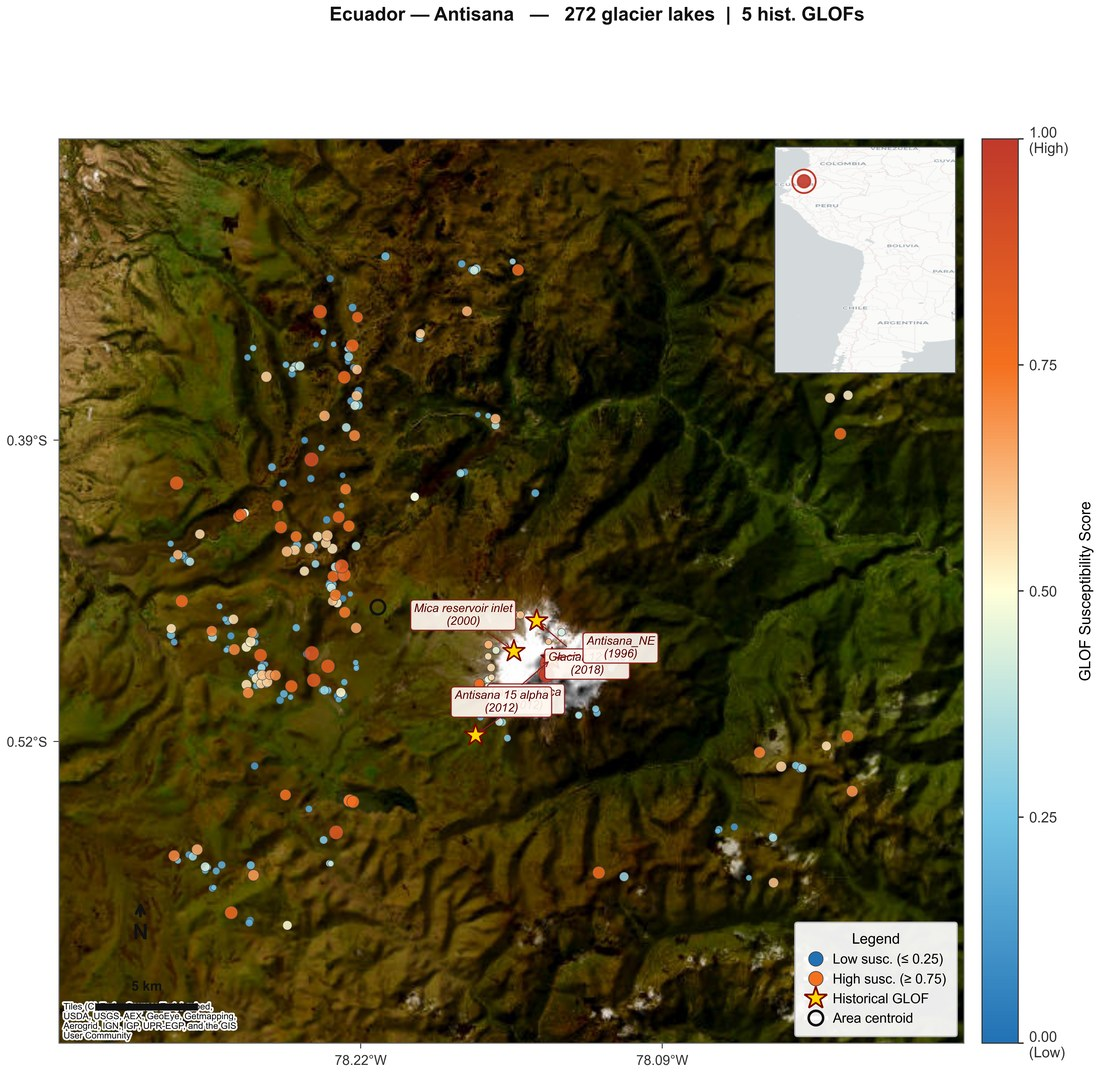
\includegraphics[width=0.31\textwidth,keepaspectratio]{areas/fig_area_ecuador.jpg}}%
\hfill
\subfloat[\textbf{Per\'u} --- C.~Blanca (3{,}083 lakes, 9 GLOFs)\label{fig:area_blanca}]{%
  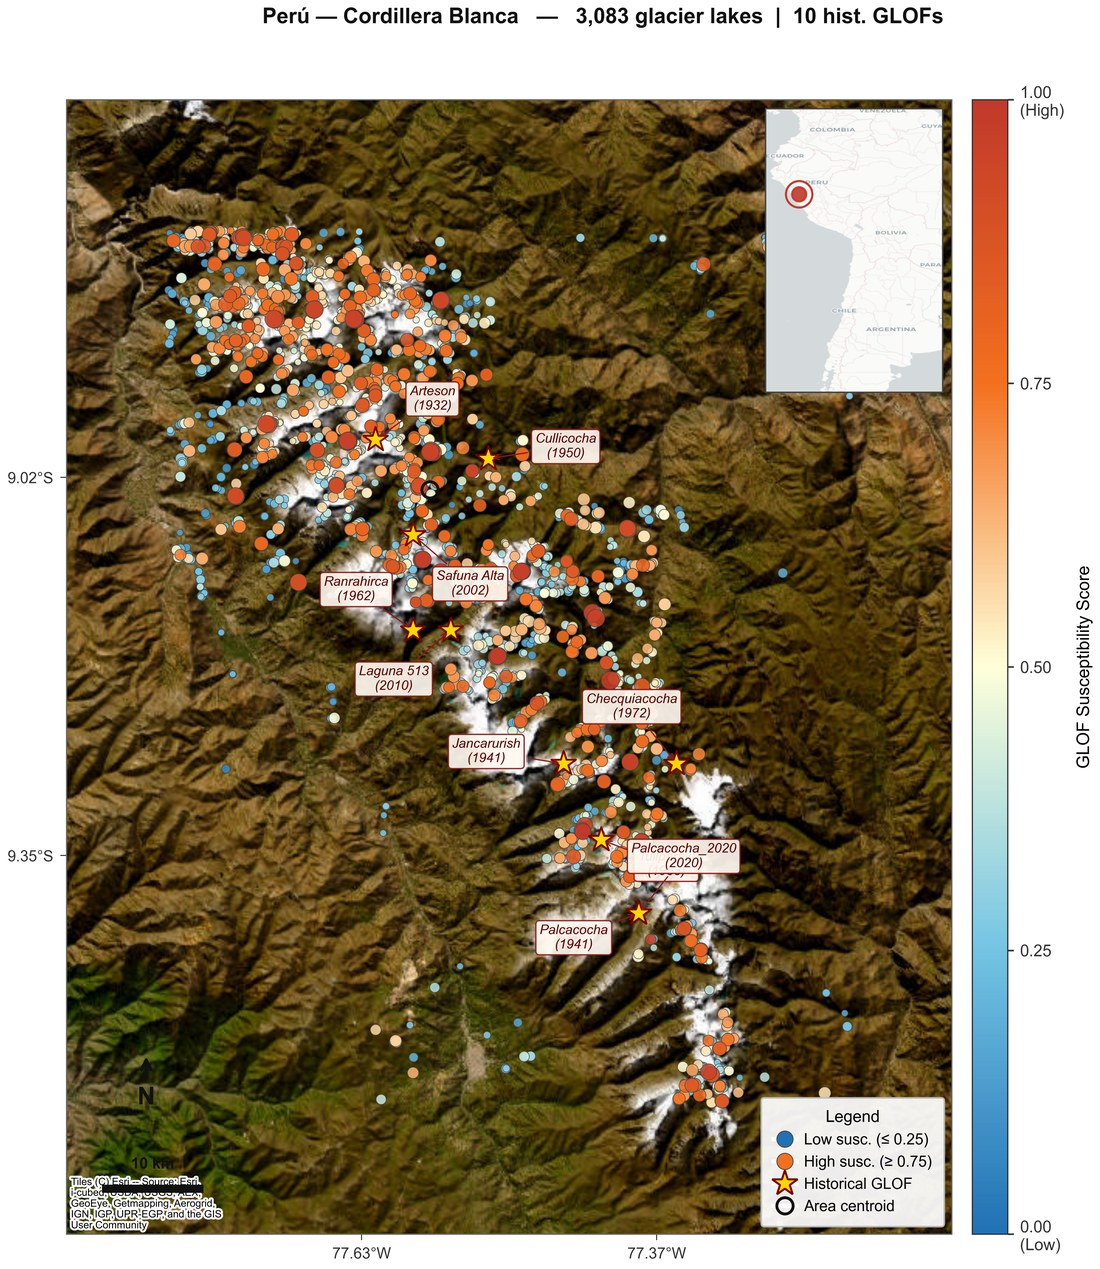
\includegraphics[width=0.31\textwidth,keepaspectratio]{areas/fig_area_peru_blanca.jpg}}%
\hfill
\subfloat[\textbf{Per\'u} --- C.~Huayhuash (278 lakes, 3 GLOFs)\label{fig:area_huayhuash}]{%
  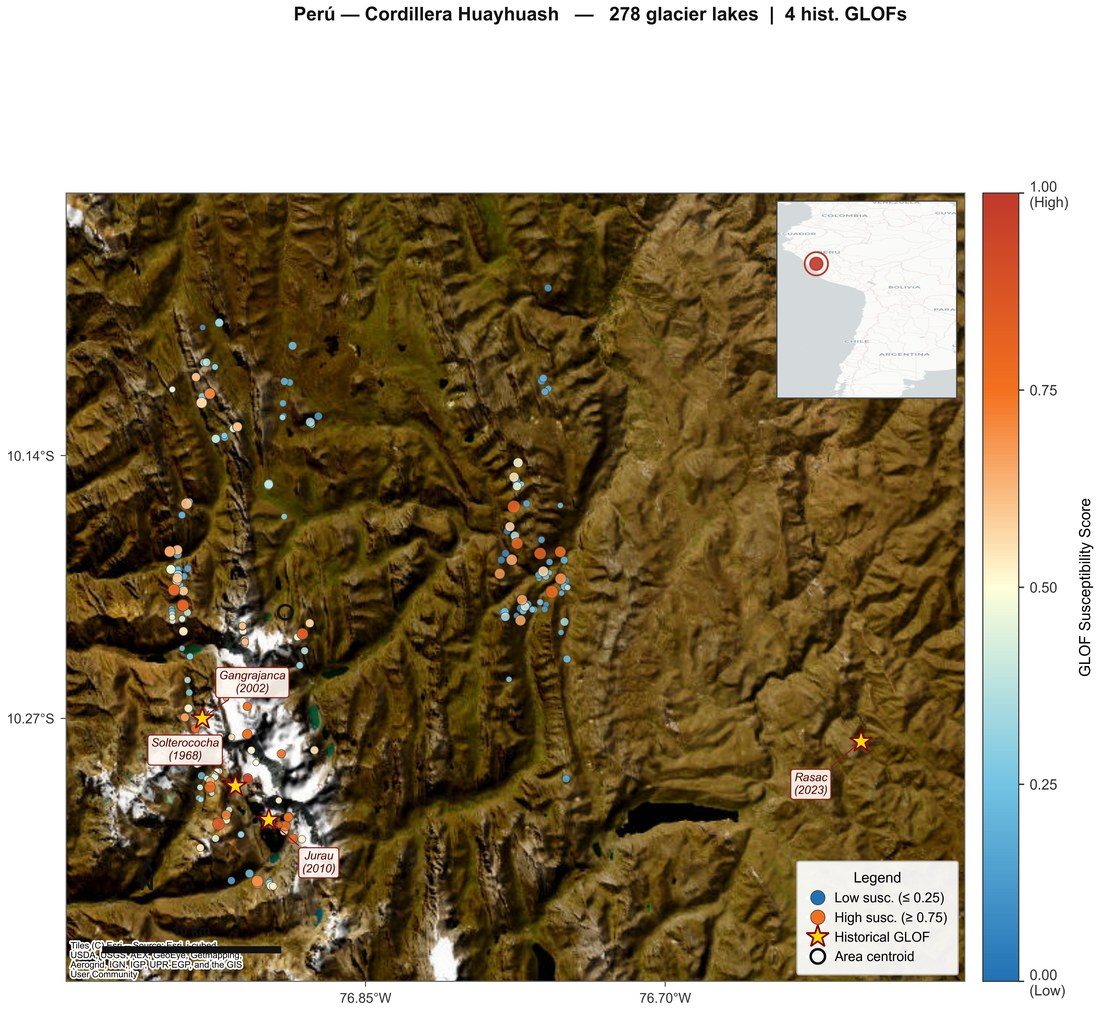
\includegraphics[width=0.31\textwidth,keepaspectratio]{areas/fig_area_peru_huayhuash.jpg}}%
\\[3pt]
%-- row 2 --
\subfloat[\textbf{Per\'u} --- C.~Raura (1{,}361 lakes, 2 GLOFs)\label{fig:area_raura}]{%
  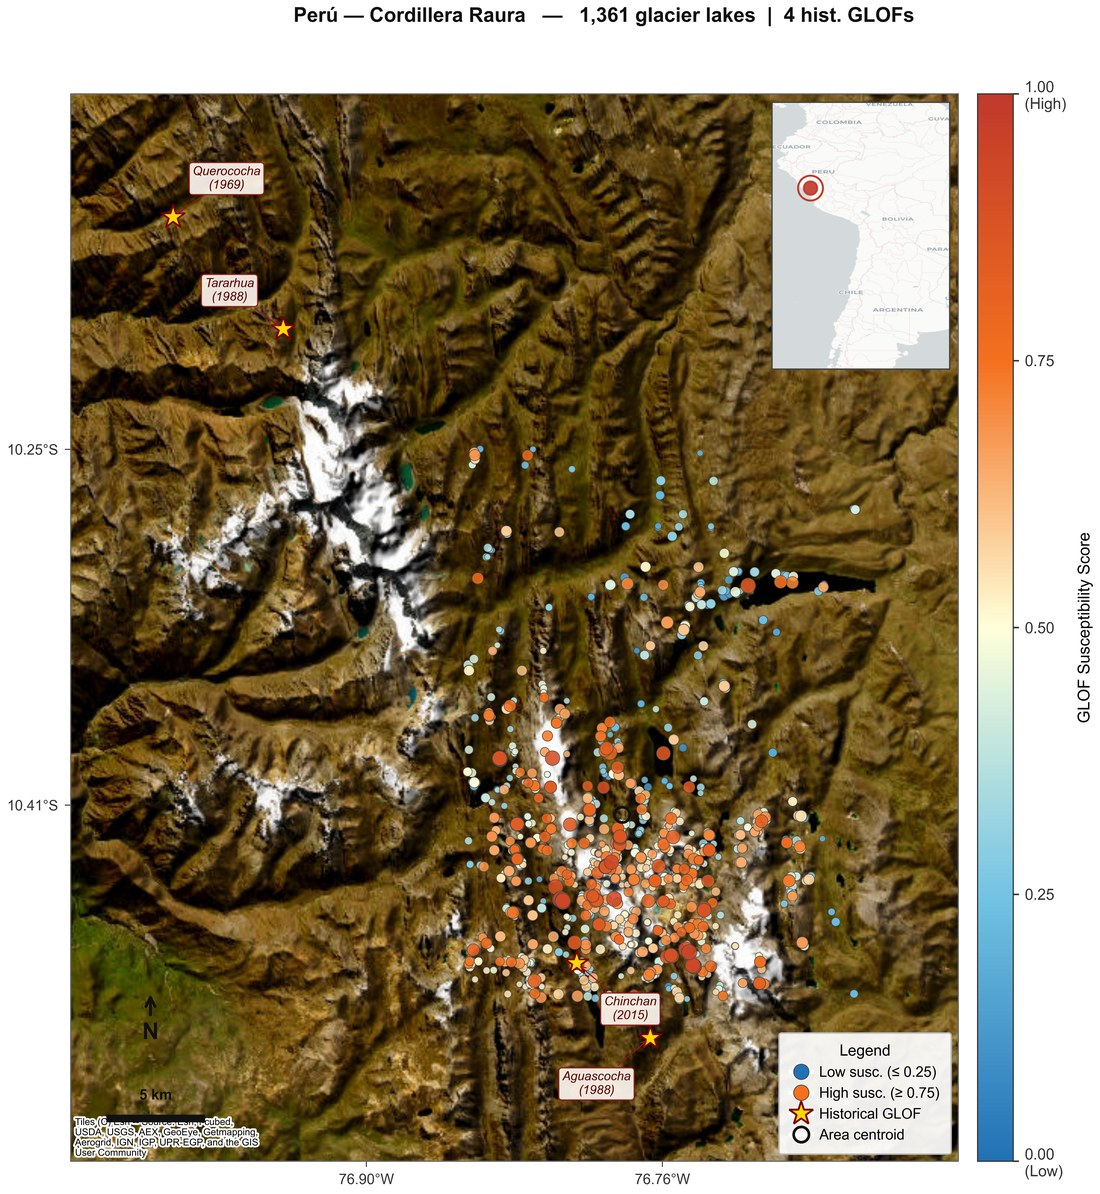
\includegraphics[width=0.31\textwidth,keepaspectratio]{areas/fig_area_peru_raura.jpg}}%
\hfill
\subfloat[\textbf{Per\'u} --- C.~Central (2{,}239 lakes, 0 GLOFs)\label{fig:area_central}]{%
  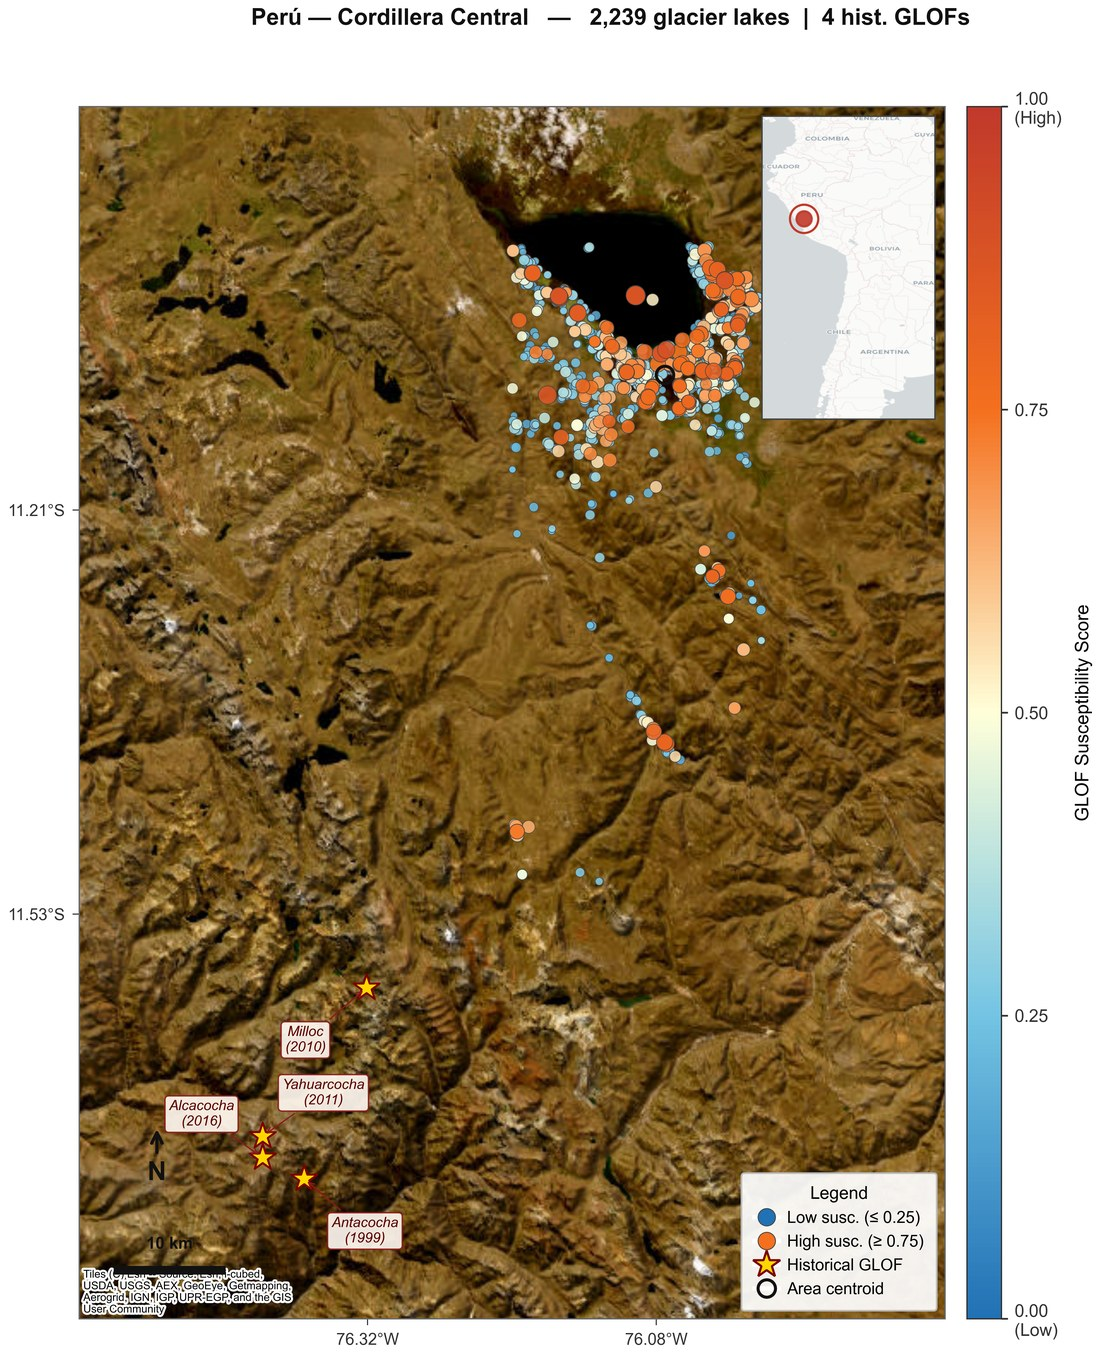
\includegraphics[width=0.31\textwidth,keepaspectratio]{areas/fig_area_peru_central.jpg}}%
\hfill
\subfloat[\textbf{Per\'u} --- C.~Urubamba (430 lakes, 0 GLOFs)\label{fig:area_urubamba}]{%
  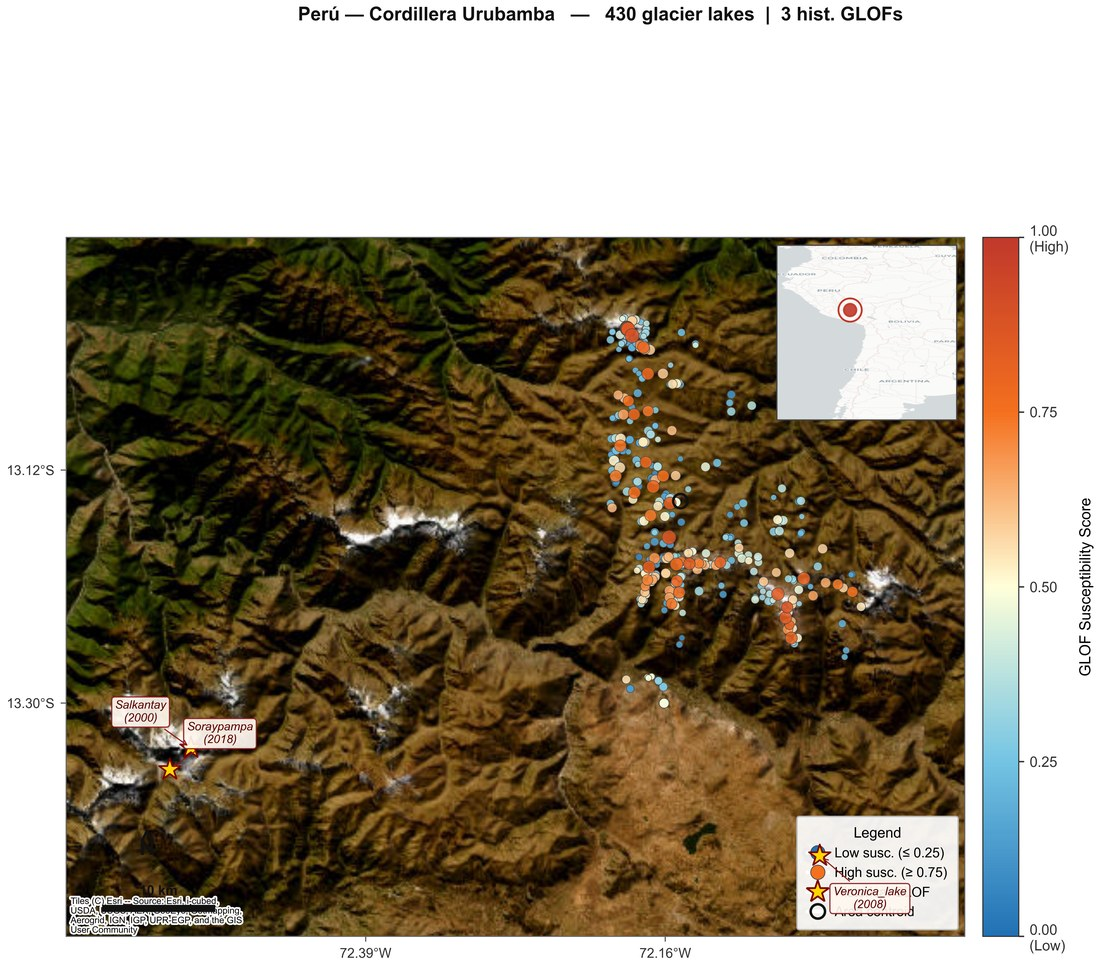
\includegraphics[width=0.31\textwidth,keepaspectratio]{areas/fig_area_peru_urubamba.jpg}}%
\caption{Study-area zoom maps (1 of 2). Symbology as described in
  Appendix~\ref{app:area_maps}.}
\label{fig:area_maps_1}
\end{figure}

\begin{figure}[!htbp]
\centering
%-- row 1 --
\subfloat[\textbf{Per\'u} --- C.~Vilcanota (2{,}770 lakes, 0 GLOFs)\label{fig:area_vilcanota}]{%
  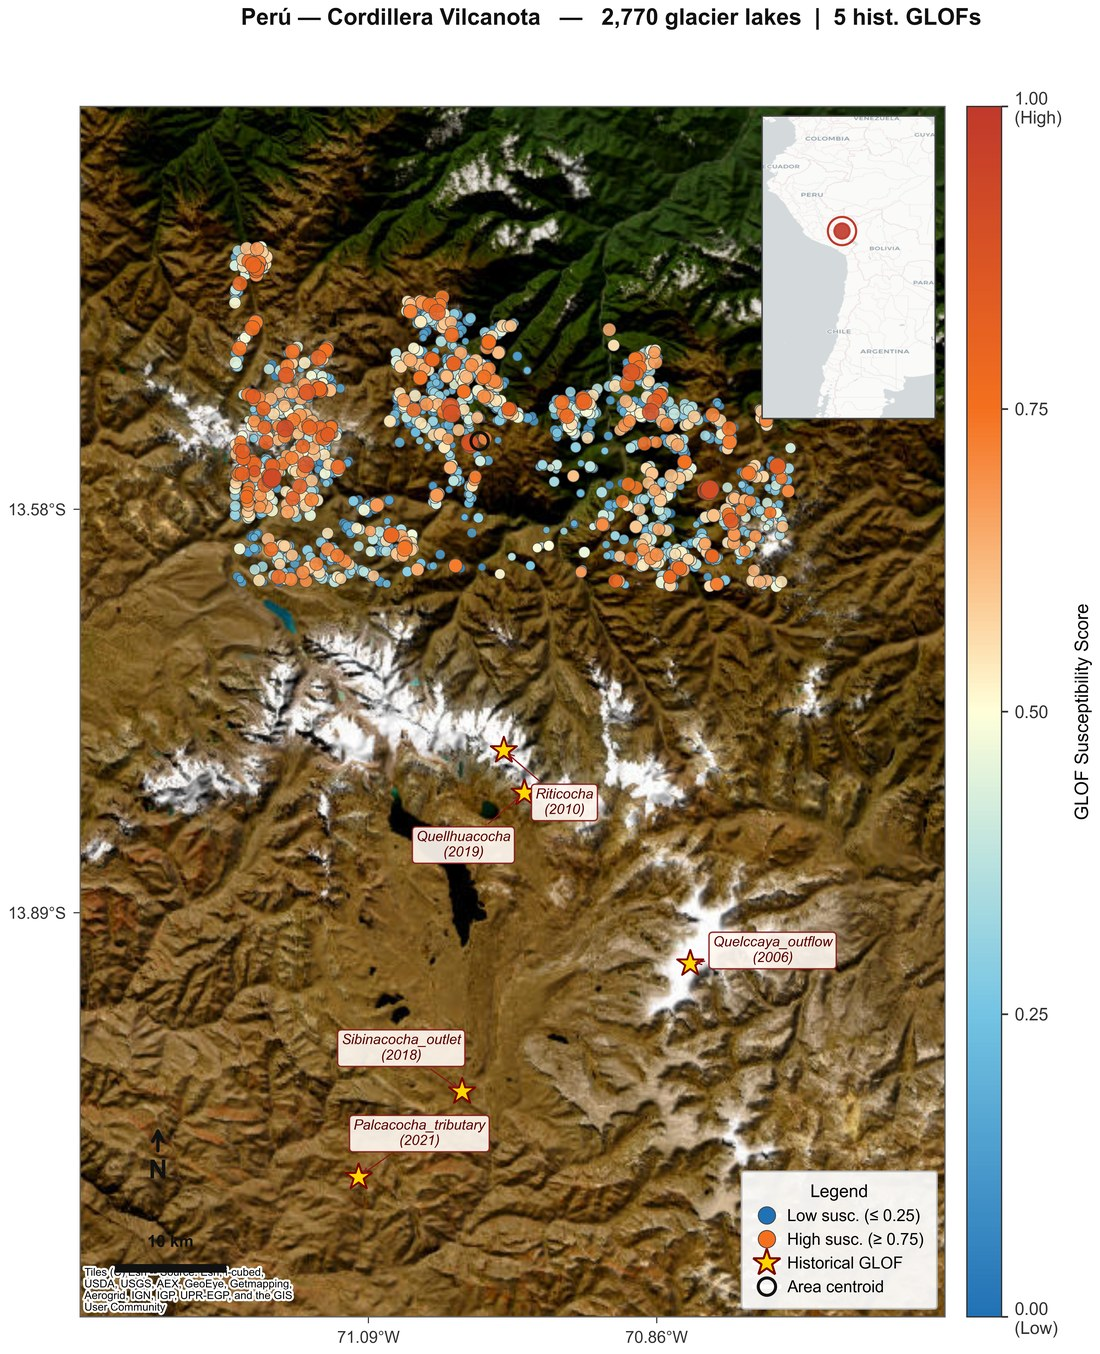
\includegraphics[width=0.31\textwidth,keepaspectratio]{areas/fig_area_peru_vilcanota.jpg}}%
\hfill
\subfloat[\textbf{Per\'u} --- C.~Huanzo (496 lakes, 0 GLOFs)\label{fig:area_huanzo}]{%
  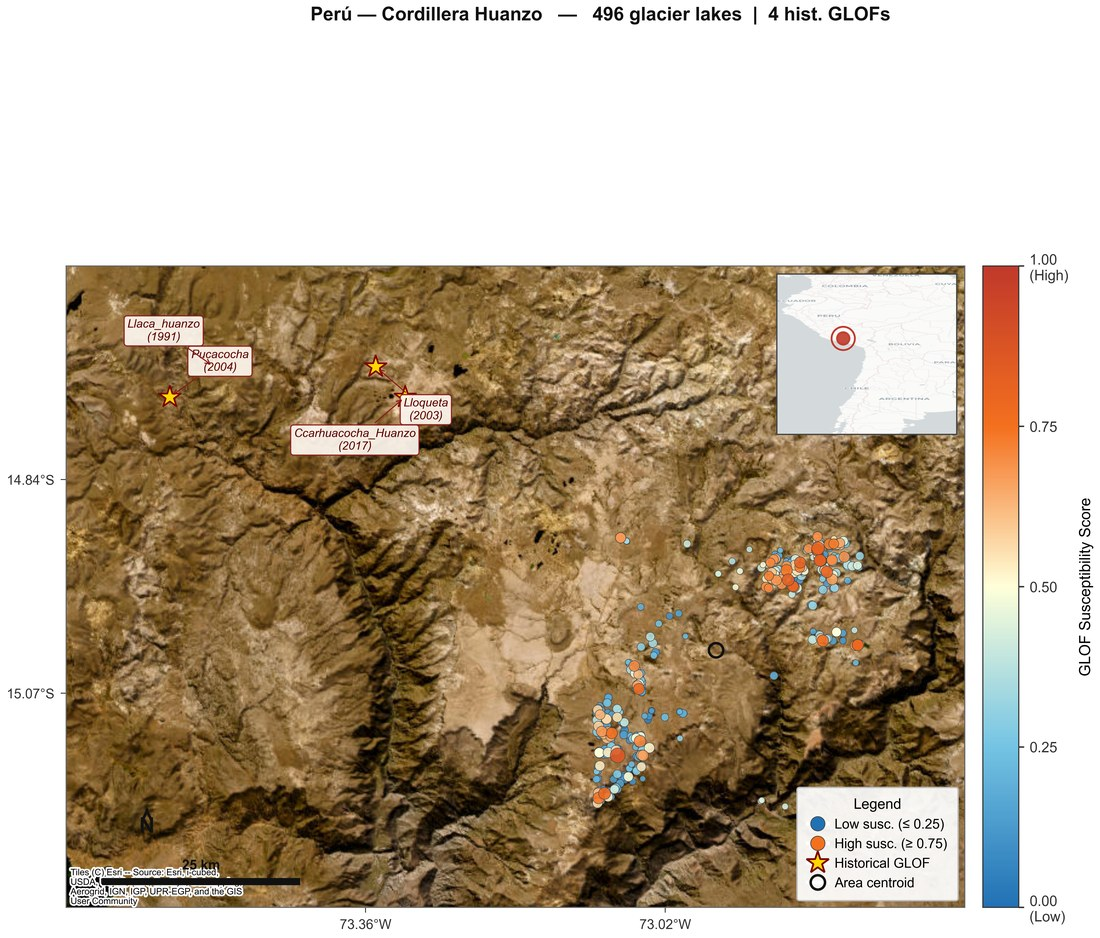
\includegraphics[width=0.31\textwidth,keepaspectratio]{areas/fig_area_peru_huanzo.jpg}}%
\hfill
\subfloat[\textbf{Bolivia} --- C.~Real (108 lakes, 1 GLOF)\label{fig:area_bolivia}]{%
  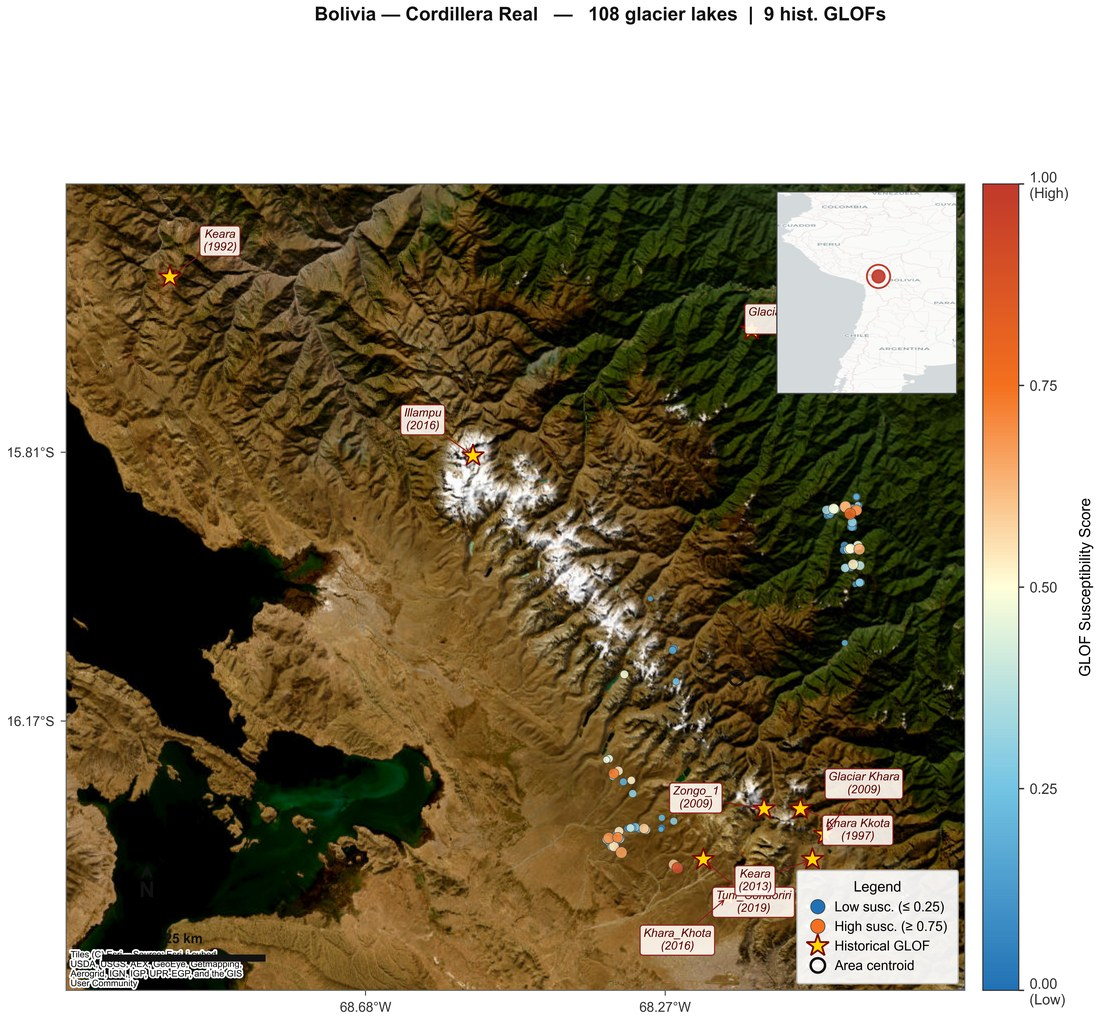
\includegraphics[width=0.31\textwidth,keepaspectratio]{areas/fig_area_bolivia.jpg}}%
\\[3pt]
%-- row 2 --
\subfloat[\textbf{Chile} --- Andes Centrales (1{,}559 lakes, 0 GLOFs)\label{fig:area_chile}]{%
  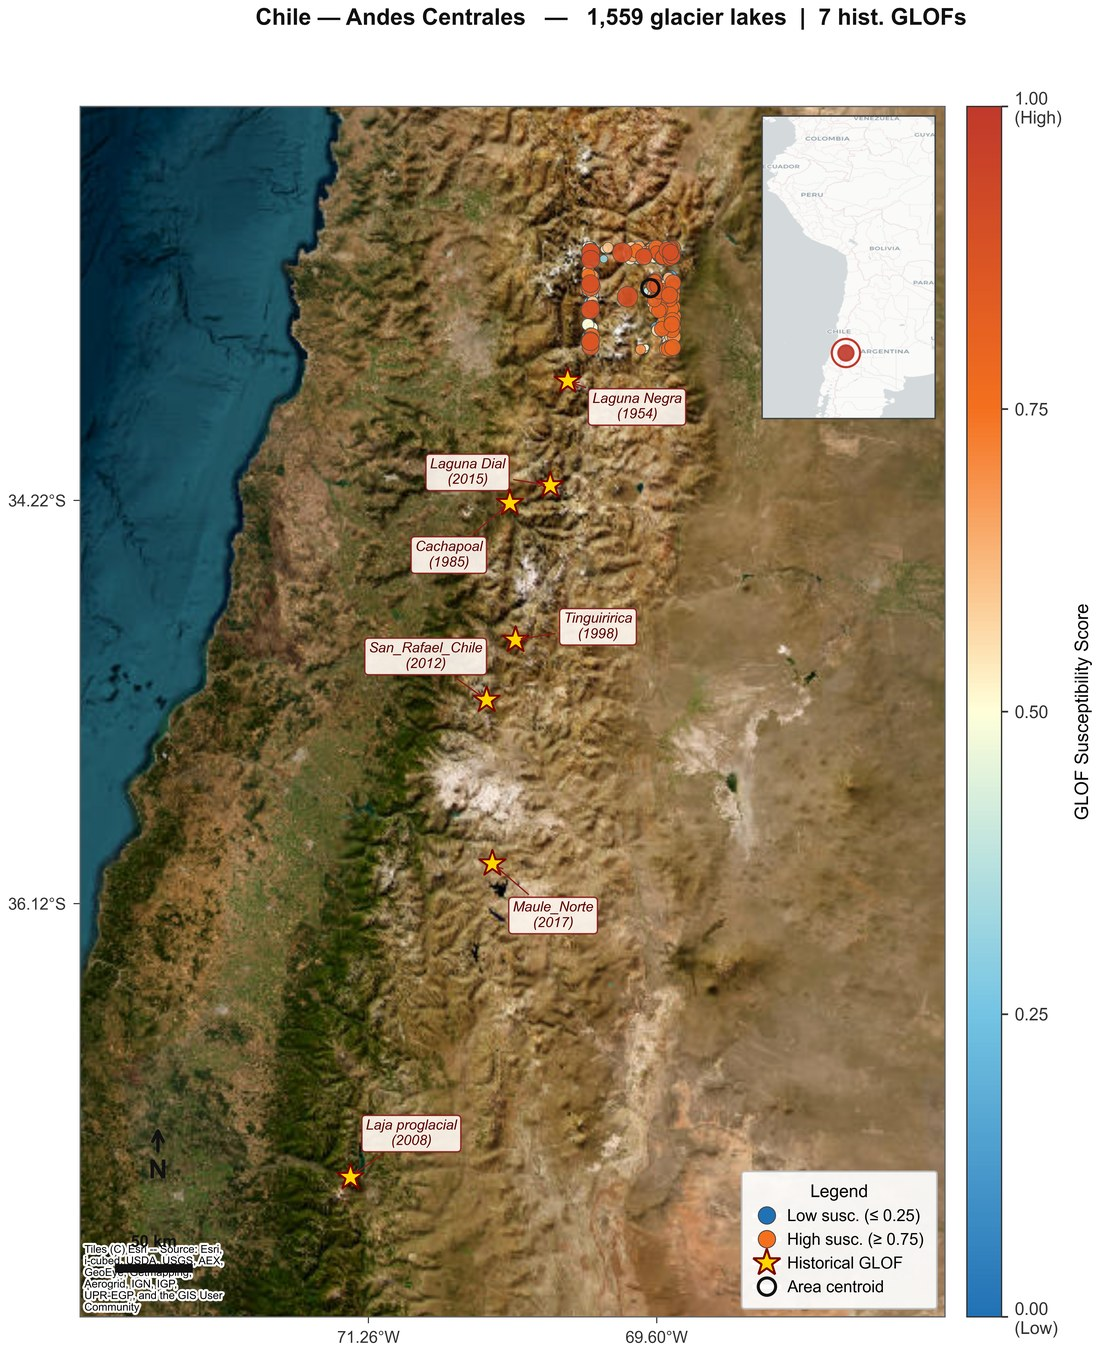
\includegraphics[width=0.45\textwidth,keepaspectratio]{areas/fig_area_chile.jpg}}%
\hfill
\subfloat[\textbf{Per\'u} --- C.~Carabaya (87 lakes, 1 GLOF)\label{fig:area_carabaya}]{%
  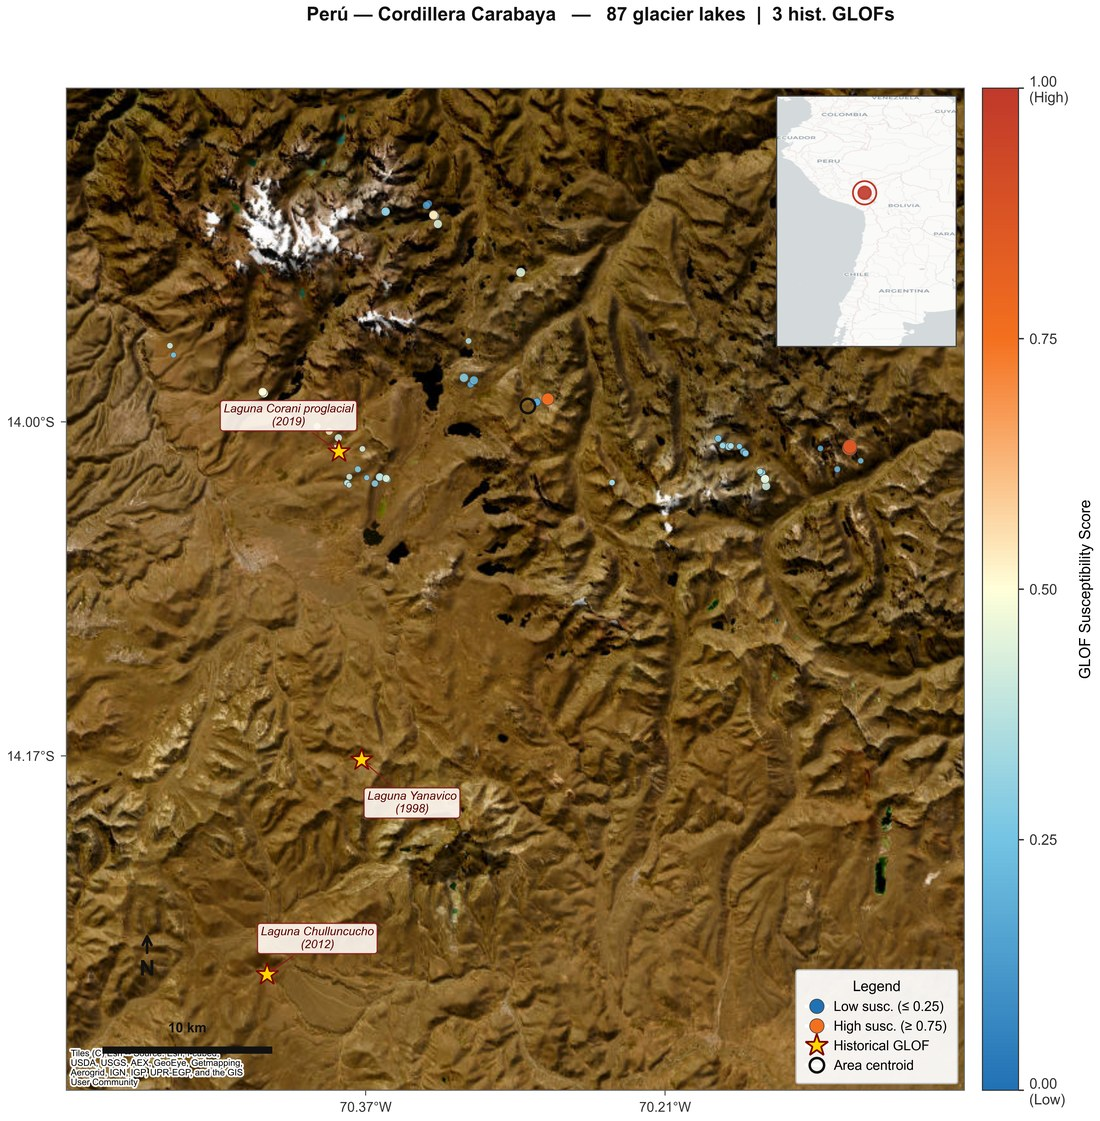
\includegraphics[width=0.45\textwidth,keepaspectratio]{areas/fig_area_peru_carabaya.jpg}}%
\caption{Study-area zoom maps (2 of 2). Symbology as in
  Fig.~\ref{fig:area_maps_1}.
  Note for Chile (Andes Centrales): historical GLOF events from the compiled
  inventory appear as stars in the map, but none spatially matched a
  detected lake within the 5\,km buffer criterion; accordingly,
  $n^+\!=\!0$ for Chile in the LOCO analysis (Table~\ref{tab:loco}).}
\label{fig:area_maps_2}
\end{figure}

\end{appendices}

%% =============================================================================
\bibliography{references_glof}

\end{document}
